\chapter{Θεωρητικό Υπόβαθρο} % Main chapter title
\label{chap:Chapter3} % For referencing the chapter elsewhere, use \ref{Chapter1} 
\epigraph{''Let no one ignorant of geometry enter” }{\textit{Plato}}

O χώρος των \Abbr{WSN} έχει και αυτός τα τελευταία χρόνια υψηλό ερευνητικό ενδιαφέρον.
Θα μπορούσε να πει κανείς - λόγο το ότι αποτελεί ένα πιο γενικό κλάδο - περισσότερο από ότι αυτό των 
drones. Συνεπώς θα μεταφερθούμε σε πρώτο επίπεδο στο πιο γενικό φάσμα, αυτό των \Abbr{WSN} 
για να προσεγγίσουμε το localization problem. 

Όταν μιλάμε για \Abbr{WSN}, αναφερόμαστε σε αυτόνομα ηλεκτρονικά συστήματα, χωρικά διασκορπισμένα σε ένα πεδίο - τα οποία συχνά περιλαμβάνουν
αισθητήρες και επικοι\-νωνούν με τα γειτονικά τους ή \Abbr{BS} για να μεταφέρουν πληροφορία \cite{wsn-wikipedia} \cite{farooqiazam2016location}.

Το καθένα από αυτά, τα ανεξάρτητα συστήματα, ονομάζεται \textbf{Node}. Ενώ, για το κάθε μεμονωμένο node - 
μπορεί να έχουμε στην διάθεση μας location information ή όχι. 
Μία πρώτη σκέψη θα ήταν, κάθε node ενός συστήματος αισθητήρων να περιλαμβάνει \Abbr{GPS} ώστε να γνωρίζουμε 
την θέση του. Αυτό μπορεί γρήγορα να καταρριφθεί σαν σκέψη, αν αναλογιστούμε αρχικά ότι το Global Navigation Satellite System (\Abbr{GNSS})
δεν είναι διαθέσιμο σε κάθε περιβάλλον λειτουργίας\footnote{Παράδειγμα ενός να είναι οι εσωτερικοί χώροι}, όπως επίσης μπορεί να μην είναι δυνατή η χρήση του σε όλους τους κόμβους
ενός συστήματος, λόγο περιορισμών όπως το κόστος\footnote{Ειδικά για low-end-low-cost devices, μπορεί να είναι ακόμα και αποτρεπτικός παράγοντας}, μέγεθος του node \& energy consumption \cite{farooqiazam2016location}, ή ακόμα ενδεχόμενο παρατήρησης
και εντοπισμού ενός ετερογενούς - από το σύστημα μας - αντικειμένου στο οποίο δεν είμαστε σε θέση να επέμβουμε.   

Στην υπάρχουσα βιβλιογραφία \cite{farooqiazam2016location} \cite{wsn-Localization-systems} \cite{wsn-Localization-techniques} βρίσκουμε ότι
nodes των οποίων η θέση είναι γνωστή ή άμεσα υπολογίσιμη, συχνά ονομάζονται \textbf{Beacons}. Πληροφορία σχετικά με την θέση αυτών
των nodes είναι γνωστή, είτε γιατί έχουν τοποθετηθεί από εμάς σε προκαθορισμένες θέσεις, είτε μέσου ενός εξωτερικού συστήματος
όπως το \Abbr{GPS} \cite{angle-of-arrival}.
Αντίθετα κόμβοι για τους οποίους δεν έχουμε αρχικά πληροφορία της θέσης τους, ονομάζονται \textbf{Non-anchors}.
Άλλος ένας σημαντικός ορισμός, που θα πρέπει να αναφερθεί είναι ότι συχνά ονομάζουμε \textbf{Settle} nodes, 
αυτά τα οποία αρχικά δεν γνωρίζαμε την θέση τους αλλά στην συνέχεια την εκτιμήσαμε.
Στο \Tabl{nodes-names-definition} παρουσιάζονται συνοπτικά τα διάφορα ονόματα που έχουν δοθεί ανά 
καιρούς για το κάθε τύπο node.

\begin{table}[H]
    \caption{Ορισμοί ονομάτων των Nodes}
    \label{tab:nodes-names-definition}
	\centering
	\resizebox{.8\textwidth}{!}{
		\begin{tabular}{ll}
			\toprule
			\textbf{Node name} & \textbf{Περιγραφή}  \\
			\midrule
				Unknown/Free/Dumb/Non-anchors & Κόμβοι με άγνωστη θέση \\
				Beacons/Anchors/Landmarks & Κόμβοι με γνώση της θέσης τους \\
				Settled & \vtop{\hbox{\strut Κόμβοι που αρχικά δεν γνωρίζαμε}\hbox{\strut την θέση τους αλλά την εκτιμήσαμε}} \\
			\bottomrule
		\end{tabular}
	}
\end{table}

Σκοπός ενός localization system είναι, με χρήση της γνώσης που έχουμε για τα beacon nodes να εκτιμήσουμε
την θέση όσο περισσότερων unknown nodes ώστε να τα μετατρέψουμε σε settled nodes και η εκτίμηση της κάθε
θέσης να είναι με όσο το δυνατόν μικρότερο error απόκλισης. 

% IMAGE
\FigCaptLabelBasedURL{../Images/Theoretical-Background/localization-systems-components.png}%
{Στοιχεία των Localization Systems}%
{Localization-Systems-components}%
<0.55>%
[wsn-Localization-systems]%
(https://ieeexplore.ieee.org/document/4407221)

Οι συγγραφείς του \cite{wsn-Localization-systems} επιχειρούν να χωρίσουν ένα localization system, ώστε 
αυτό να αποτελείται από τρία διακριτά components, αυτή τη κατηγοριοποίηση την υιοθετούν κατά την έρευνα τους και οι ερευνητές του \cite{localization-systems-components}. Πρώτο μπορεί να θεωρηθεί αυτό του \textbf{Distance/Angle Estimation}, 
που σκοπό έχει να υπολογίσει την γωνία ή απόσταση που έχουν δύο nodes του συστήματος μεταξύ τους.
Η πληροφορία που θα παραχθεί από αυτό το component θα χρησιμοποιηθεί στα άλλα μέρη του συστήματος.
Στην συνέχεια υπάρχει το \textbf{Position Computation}, δουλειά του οποίου είναι να υπολογίσει την θέση ενός
node με βάση την γνώση που έχουμε για τα beacons και την πληροφορία που λάβαμε από το πρώτο component.
Ενώ τέλος είναι το κύριο μέρος του συστήματος, με όνομα \textbf{Localization Algorithm} και ουσιαστικά είναι
ο προκαθορισμένος τρόπος που θα ακολουθηθεί για να υπολογιστεί η θέση των unknown nodes με βάση όλες τις 
πληροφορίες που έχουμε.
Στην \Fig{Localization-Systems-components} δίνεται η απεικόνιση που έδωσαν οι συγγραφείς του 
\cite{wsn-Localization-systems} για να εξηγήσουν το παραπάνω. Ενώ στην \Fig{Localization-system}
έχει γίνει μία προσπάθεια να κατηγοριοποιηθούν τα κομμάτια καθώς και τεχνικές των Localization Systems,
με βάση τα \cite{farooqiazam2016location} \cite{wsn-Localization-systems} \cite{wsn-Localization-techniques}
και αναλύονται στην συνέχεια του κεφαλαίου.

\begin{figure} [H]
	\tikzset{
		basic/.style  = {draw, text width=2cm, font=\sffamily},
		root/.style   = {basic, thin, align=center, fill=white, text width=5cm},
		level 1/.style = {sibling distance=16em, level distance=5em},
		level-2/.style = {basic, thin, align=center, fill=white, text width=5.5cm},
		level-31/.style = {basic, thin, align=center, fill=white, text width=2cm},
		level-32/.style = {basic, thin, align=center, fill=white, text width=2.8cm},
		level-33/.style = {basic, thin, align=center, fill=white, text width=5cm},
		level-4/.style = {basic, thin, align=center, fill=white, text width=4.5cm},
		level-42/.style = {basic, thin, align=center, fill=white, text width=4.8cm},
		edge from parent/.style={->,solid,black,thick,draw}, 
		edge from parent path={(\tikzparentnode.south) -- (\tikzchildnode.north)},
		>=latex, node distance=1.5cm, edge from parent fork down
	}
	\centering
	\resizebox{.9\textwidth}{!}{
		\begin{tikzpicture}[]
			\node[root] {\textbf{Localization Systems}}
				child {node[level-2] (c1) {\textbf{Distance/Angle Estimation}}}
				child {node[level-2] (c2) {\textbf{Position Computation}}}
				child {node[level-2] (c3) {\textbf{Localization Algorithm}}};
			
			% -----------------------------------------------------------------------------
			% Distance/Angle
			\node [level-31, below of = c1, xshift=-25pt] (c11) {Distance};
				\node [level-4, below of = c11, xshift=50pt] (c111) {Received Signal Strength};
				% \node [level-4, below of = c111] (c112) {Lighthouse approach};
				\node [level-4, below of = c111] (c113) {Propagation time based measurements};
					\node [level-42, below of = c113, xshift=30pt] (c1131) {One-way propagation time};
					\node [level-42, below of = c1131] (c1132) {Roundtrip propagation time};
					\node [level-42, below of = c1132] (c1133) {Time Difference of Arrival};
					\foreach \value in {1,2,3} \draw[->] (c113.197) |- (c113\value.west);
				\foreach \value in {1,3} \draw[->] (c11.195) |- (c11\value.west);

			\node [level-31, below of = c1133, xshift=-80pt] (c12) {Angle};
				\node [level-4, below of = c12, xshift=70pt] (c121) {Receiver Antenna Amplitude response};
				\node [level-4, below of = c121] (c122) {Receiver Antenna Phase response};
				\foreach \value in {1,2} \draw[->] (c12.210) |- (c12\value.west);
			\foreach \value in {1,2}   \draw[->] (c1.188) |- (c1\value.west);
			
			% Position Computation
			\node [level-32, below of = c2, xshift=25pt] (c21) {Trilateration};
			\node [level-32, below of = c21] (c22) {Bounding box};
			\node [level-32, below of = c22] (c23) {Triangulation};
			\node [level-32, below of = c23] (c24) {Multilateration};
			\node [level-32, below of = c24] (c25) {Probabilistic approaches};
			\node [level-32, below of = c25] (c26) {Central position};
			\foreach \value in {1,...,6} \draw[->] (c2.196) |- (c2\value.west);

			% Localization Algorithm
			\node [level-33, below of = c3, xshift=10pt] (c31) {Range-based/Range-free};
			\node [level-33, below of = c31] (c32) {Distributed/Centralized \\ Position Computation};
			\node [level-33, below of = c32] (c33) {Relative/Absolute Positioning};
			\node [level-33, below of = c33] (c34) {Indoor/Outdoor scenarios};
			\node [level-33, below of = c34] (c35) {One-hop/Multihop};
			\node [level-33, below of = c35] (c36) {With/Without Infrastructure};
			\node [level-33, below of = c36] (c37) {Anchor Based/Free};
			\foreach \value in {1,...,7} \draw[->] (c3.187) |- (c3\value.west);
		\end{tikzpicture}
	}
	\decoRule
	\caption[Επισκόπηση των Localization System (RF-based approach)]{Επισκόπηση των Localization System (\Abbr{RF}-based approach)}
	\label{fig:Localization-system}
\end{figure}

Με βάση τον παραπάνω διαχωρισμό των Localization Systems σε τρία διακριτά μέρη, μπορούμε να καταλάβουμε
ότι η απόκλιση της εκτίμησης του συνολικού συστήματος, εξαρτάται από τα σφάλματα  του κάθε μεμονωμένου μέρους.

Τέλος, έχει γίνει ήδη αναφορά ότι το πρόβλημα προσδιορισμού της θέσης ενός α\-ντι\-κει\-μέ\-νου, μπορεί να προσεγγιστεί με χρήση διαφορετικών μεθόδων,
με αυτές να μπορούν να κατηγοριοποιηθούν σε τεχνικές που σχετίζονται με ενέργεια (e.g. \Abbr{RF} and sound)
και τεχνικές που σχετίζονται με οπτικά μέσα\footnote{Ενώ κάποιες φορές μπορούν να συνδυαστούν βασικές αρχές της κάθε μία για μία ενοποιημένη υλοποίηση}. Στην συνέχεια του κεφαλαίου, γίνεται διαδοχική αναφορά στην κάθε μία εξ' αυτών.  

%----------------------------------------------------------------------------------------
%	SECTION 1
%----------------------------------------------------------------------------------------
\section{Εντοπισμός θέσης με βάση την ενέργεια} \label{sec:Energy-based} 

\subsection{Εκτίμηση Απόστασης/Γωνίας}\label{sec:Distance-Angle-Estimation}

Θα ξεκινήσουμε με μία σύντομη ανάλυση των τεχνικών εκτίμησης της απόστασης - μεταξύ δύο nodes -
που χρησιμοποιούνται ήδη, στις προσεγγίσεις \Abbr{RF} \& sound. 

%----------------------------------------------------------------------
\subsubsection{Received Signal Strength}
Η πρώτη τεχνική η οποία έχει χρησιμοποιηθεί για τον υπολογισμό απόστασης στα 
\Abbr{WSN} (χρήση \Abbr{RF}), είναι αυτή με όνομα Received Signal Strength Indicator
(\Abbr{RSSI}) και έχει ως αρχή την χρήση της έντασης της ισχύς ενός 
σήματος που λαμβάνουμε στον δέκτη, ως τρόπο υπολογισμού της απόστασης
του πομπό από αυτόν. Path loss ή path attenuation \cite{wikipedia-Path_loss} ονομάζεται η μείωση της ισχύς
ενός σήματος καθώς αυτό διαδίδεται.
Στον ελεύθερο χώρο η λαμβανόμενη ισχύς $P_r(d)$ που ανιχνεύει ο πομπός
μπορεί να περιγραφτεί από το μοντέλο του Free Space Path Loss (\Abbr{FSPL}) \cite{wikipedia-fspl}, το οποίο προκύπτει
μέσω της Friis transmission equation \cite{wsn-Localization-techniques} \cite{rssi-wlan} \cite{wikipedia-friis-equation} - σχέση \EqNum{signal-strength}.

\begin{align}
	P_r(d)=\frac{P_tG_tG_r\lambda^2}{(4\pi)^2d^2} \label{eq:signal-strength}
\end{align}

Όπου $P_t$ είναι η ισχύς που στέλνει ο πομπός, $G_t$ είναι το gain της κεραίας του
πομπού, $G_r$ το gain της κεραίας του δέκτη, λ είναι το μήκος κύματος του σήματος
το οποίο μεταδίδουμε και d η απόσταση του πομπού από τον δέκτη. Αν θεωρήσουμε ότι 
τα $G_t$, $G_r$ και λ είναι μη μεταβλητές τιμές - με $C_f = \frac{G_tG_r\lambda^2}{(4\pi)^2}$ - τότε μπορούμε να καταλήξουμε
στην \EqNum{signal-strength-simple} \cite{rssi-simple-formula}.

\begin{align}
	P_r(d)=C_f\frac{P_t}{d^2} \label{eq:signal-strength-simple}
\end{align}

Αυτό που μπορούμε να δούμε από την παραπάνω σχέση είναι ότι, ιδανικά στον ελεύθερο 
χώρο σε Line of Sight (\Abbr{LoS}) μετάδοση -
η ισχύς του σήματος που λαμβάνει ο πομπός εξαρτάται από το αντίστροφο τετράγωνο της
απόστασης των δύο nodes. Η σχέση \EqNum{signal-strength-simple} συχνά αναφέρεται σε watt, 
όμως όταν μιλάμε για transmitting power αντί για την χρήση των watt, είναι αρκετά βολική
η χρήση του dBm \cite{wikipedia-dBm}. Για αυτό το λόγο, παρακάτω παρουσιάζονται τα conversion
equations, από το ένα στο άλλο \cite{rssi-wlan} \cite{wikipedia-dBm}. 

\begin{align}
	\left\{
		\begin{array}{ll}
			P[dBm]= 10\cdot log_{10}\left(\frac{P[mW]}{1[mW]}\right) \\[10pt]
			\quad \quad P[mW] = 10^\frac{(P[dBm])}{10}
		\end{array}
	\right.
\end{align}

Ενώ η \Fig{Ideal-RSSI-over-distance} περιγράφει σχηματικά το ιδανικό μοντέλο της εξάρτηση της ισχύς με την αύξηση
της απόστασης όταν χρησιμοποιούμε στον δέκτη μέτρηση σε dΒm. 

%-------------------------------------------

\FigCaptLabelBasedURL{../Images/Theoretical-Background/Ideal-RSSI-over-distance.png}%
{Ideal RSSI over distance}%
{Ideal-RSSI-over-distance}%
<0.35>%
[ideal-rssi-model]%
(https://www.semanticscholar.org/paper/Adaptive-Distance-Estimation-Based-on-RSSI-in-802-.-Botta-Simek/8b7669850aecaa7b4f8a1b774f260bff24b20ef6)

Αν λοιπόν, μετράμε την ισχύ με την οποία λαμβάνουμε ένα σήμα, μπορούμε να είμαστε σε θέση να υπολογίσουμε την απόσταση που βρίσκεται
ο πομπός από εμάς.
Αυτή η μέθοδος παρόλο που είναι αρκετά δημοφιλής και οικονομική για τον υπολο\-γισμό της απόστασης
- λόγω του ότι δεν απαιτεί επιπλέον αισθητήρες - σε πρα\-γματικές 
συνθήκες αντιμετωπίζει αρκετά προβλήματα, καθώς οι μετρήσεις μπορούν να επηρεαστούν από θόρυβο,
ανακλάσεις του σήματος, διαθλάσεις, δυναμικά περιβάλλοντα ή εμπόδια σε αυτά, Non-Line of Sight (\Abbr{NLoS}) μετάδοση, 
ή ακόμα και errors στο hardware 
\cite{wsn-Localization-systems} \cite{ideal-rssi-model}.
Σε ένα βαθμό μπορεί να βελτιωθεί η απόδοση με στατικό ή δυναμικό calibration του συστήματος,
όμως μέχρι τώρα δεν χρησιμοποιείται για εκτίμηση απόστασης σε εφαρμογές όπου nodes έχουν μεγάλη
απόσταση μεταξύ τους ή μας ενδιαφέρει να έχουμε μεγάλη ακρίβεια προσέγγισης της απόστασης \cite{ideal-rssi-model}.

%----------------------------------------------------------------------
\subsubsection{Propagation Time}
Σε αυτήν την κατηγορία εκτίμησης απόστασης μεταξύ nodes - η οποία βασίζεται σε χρονικές μετρήσεις της διάδοσης του σήματος,
 Time of Flight (\Abbr{ToF})
- κατά κύριο λόγο χρησιμοποιούνται δύο βασικές τεχνικές, η Time of Arrival (\Abbr{ToA}) και η Time 
Difference of Arrival (\Abbr{TDoA}) \cite{wsn-Localization-systems}. 

Θα ξεκινήσουμε με μία σύντομη περιγραφή της \Abbr{ToA}. Από την κινηματική γνωρίζουμε την 
σχέση \EqNum{speed}, η οποία συσχετίζει την ταχύτητα κίνησης ενός σώματος \emph{V} ως το πηλίκο της μεταβολής
της θέσης $\mathrm{d}s$ - που έκανε το σώμα, προς τον χρόνο $\mathrm{d}t$ που χρειάστηκε για να πραγματοποιηθεί η μεταβολή \cite{Kinematics}.

\begin{gather}
	V=\frac{\mathrm{d}s}{\mathrm{d}t} \label{eq:speed} \\
	d=s(t_b-t_a) \label{eq:tod-distance}
\end{gather}

Αξιοποιώντας την \EqNum{speed} ως αρχή, μπορούμε να καταλήξουμε στην \EqNum{tod-distance} για να εκτιμήσουμε
την απόσταση \emph{d} που βρίσκονται δύο nodes μεταξύ τους, αν ένα κύμα κινείται με ταχύτητα \emph{s} και χρειάστηκε 
χρόνο \emph{t} για να μεταδοθεί από το ένα node στο άλλο. Στην \Fig{Time-of-Arrival-cases} (a) απεικονίζεται
σχηματικά αυτό, όπου $t=t_b-t_a$ με $t_b$ η χρονική στιγμή που φτάνει το κύμα στο receiver και $t_a$
η χρονική στιγμή η οποία ξεκινάει από τον transmitter. Σε περίπτωση που μιλάμε για  
\Abbr{RF} η ταχύτητα μετάδοσης του κύματος είναι ίση με την ταχύτητα μετάδοσης του φωτός $c_o$, το οποίο 
σε $0.1μs$ διανύει περίπου $30m$.   
Με βάση αυτό, μπορούμε εύκολα να καταλάβουμε ότι για να έχουμε ακριβή αποτελέσματα είναι αρκετά σημαντικό
τα clocks των δύο nodes να είναι απόλυτα συγχρονισμένα για να μην έχουμε error απόκλισης, πράγμα που
απαιτεί να κάνουμε το συνολικό σύστημα αρκετά πιο πολύπλοκο σχεδιαστικά 
ώστε η απόκλιση μας να είναι σε ανεκτά σημεία για την εφαρμογή \cite{wsn-Localization-systems} \cite{wsn-Localization-techniques}.

\begin{figure} [H]
    \centering
    % -----------------
    \begin{minipage}{.5\textwidth}
      \centering
      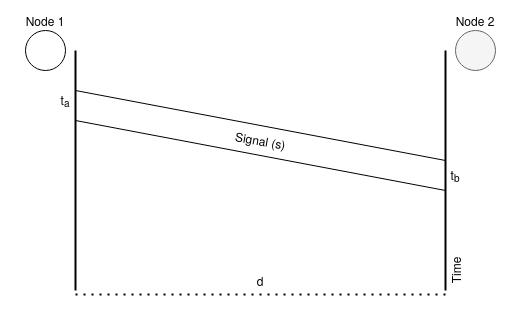
\includegraphics[width=.8\linewidth]{../Photos/toa-oneway.png}\\
      {(a) One-way}
    \end{minipage}%
    % -----------------
    \begin{minipage}{.5\textwidth}
      \centering
      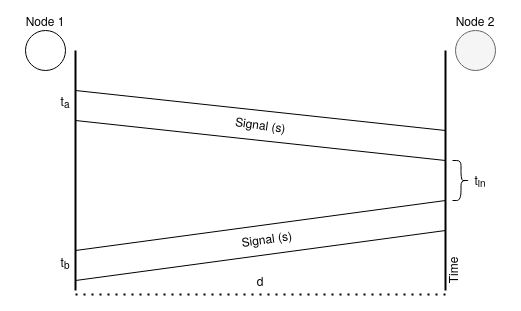
\includegraphics[width=.8\linewidth]{../Photos/toa-roundtrip.png}\\
      {(b) Roundtrip}
    \end{minipage}
    \hfill \break
    \decoRule
    \caption[Time of Arrival cases]{Time of Arrival cases}
    \label{fig:Time-of-Arrival-cases}
\end{figure}

Μπορούμε να το παρακάμψουμε αυτό, με το να γίνει η μέτρηση σε Round-Trip Time (\Abbr{RTT}), \Fig{Time-of-Arrival-cases} (b).
Σε αυτήν την περίπτωση το ένα node στέλνει ένα σήμα, και μόλις το λάβει ένα γειτονικό node, απαντάει πίσω στο πρώτο. 
Με αυτόν τον τρόπο η μέτρηση του χρόνου εκκίνησης $t_a$ και άφιξης $t_b$ του σήματος γίνονται στο ίδιο node - 
άρα δεν χρειάζεται συγχρονισμός, και η πραγματική απόσταση είναι η μισή από αυτή που θα υπολογιστεί. Ο κύριος παράγοντας
σφάλματος σε αυτή την μέθοδο, είναι ο υπολογισμός του χρόνου που χρειάστηκε το δεύτερο node για να διαχειριστεί
το σήμα που έλαβε και να απαντήσει. Αυτό το internal delay $t_{in}$ μπορεί να είναι είτε γνωστό από 
ένα a priori calibration, είτε μπορεί να μετριέται και να στέλνεται μαζί με το σήμα απάντησης - ώστε να αφαιρείται
από τον χρόνο μετάδοσης του κύματος \cite{wsn-Localization-techniques}.
Με αυτά τα δεδομένα, η σχέση \EqNum{toa-roundtrip} περιγράφει τον τρόπο υπολογισμού της
απόστασης \emph{d} μεταξύ των δύο nodes.

\begin{align}
	d=\frac{s(t_b-t_a-t_{in})}{2} \label{eq:toa-roundtrip}
\end{align}


Όσον αφορά την τεχνική \Abbr{TDoA}, και σε αυτήν την περίπτωση υπάρχουν δύο παραλλαγές της \cite{wsn-Localization-systems} - όπου και οι 
δύο είναι βασισμένες στην αρχή το ότι δεν μας ενδιαφέρει η χρονική στιγμή που ξεκίνησε η αποστολή ενός σήματος, αλλά μόνο
οι χρονική στιγμή που το λάβαμε.

\begin{figure} [H]
    \centering
	% -----------------
    \begin{minipage}{.5\textwidth}
      \centering
      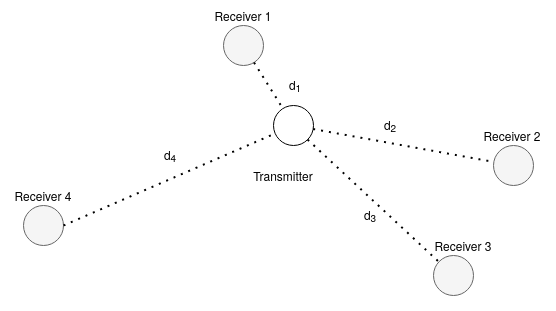
\includegraphics[width=0.8\linewidth]{../Photos/tdoa-multiple.png}\\
      {(a) Single signal - multiple receivers}
    \end{minipage}%
    % -----------------
    \begin{minipage}{.5\textwidth}
      \centering
      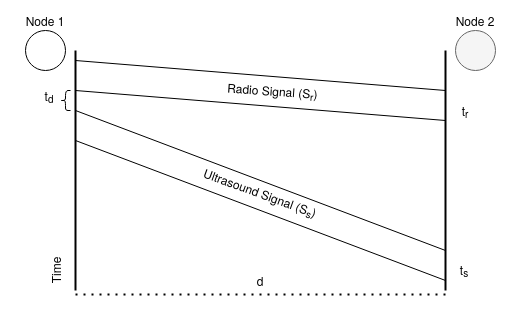
\includegraphics[width=.8\linewidth]{../Photos/tdoa-timing.png}\\
      {(b) Multiple signals - single receiver}
    \end{minipage}
    \hfill \break
    \decoRule
    \caption[Time Difference of Arrival cases]{Time Difference of Arrival cases}
    \label{fig:Time-Difference-of-Arrival-cases}
\end{figure}


Η πρώτη περίπτωση σχετίζεται με single signal και multiple receivers, παρουσιάζεται στο 
\Fig{Time-Difference-of-Arrival-cases} (a), 
χρησιμοποιείται συνήθως στα cellular network και απαιτεί την ύπαρξη 
τουλάχιστον 4 beacons για την απόκτηση location πληροφορίας ενός free node στον τρισδιάστατο χώρο. Υπολογίζει την χρονική διαφορά
που έφτασε σε καθένα από τα beacons το σήμα που έστειλε το free node, για την εκτίμηση της θέσης του free node από
το καθένα από αυτά. Σημαντικό σε αυτήν την περίπτωση είναι και εδώ, να είναι απόλυτα συγχρονισμένα τα beacons. 
Βασίζεται στις ιδιότητες των υπερβολικών καμπύλων και στο ότι με δεδομένη μία συγκεκριμένη χρονική διαφορά του σήματος, 
το free node θα πρέπει να βρίσκεται κάπου πάνω σε μία υπερβολική καμπύλη όπως παρουσιάζεται από την \Fig{TDoA-hyberbolas}
\cite{youtube-angle-of-arrival-tdoa-hyberbolas}. 

Μόνο από αυτόν τον υπολογισμό δεν δύναται να κάνουμε ακριβή εκτίμηση από\-στασης, 
μπορούμε να συμπεράνουμε όμως τον γεωμετρικό τόπο στον οποίο βρίσκεται το free node. Στη \Sect{Multilateration} - και σε επέκταση αυτού -
παρουσιάζεται όμως, ο τρόπος με τον οποίο μπορούμε να συνδυάσουμε τέτοια πληροφορία από πολλαπλά beacon για να εκτιμήσουμε την ακριβή θέση του free node.

\begin{figure} [H]
	\centering
	% -----------------
    \begin{minipage}{.5\textwidth}
      \centering
      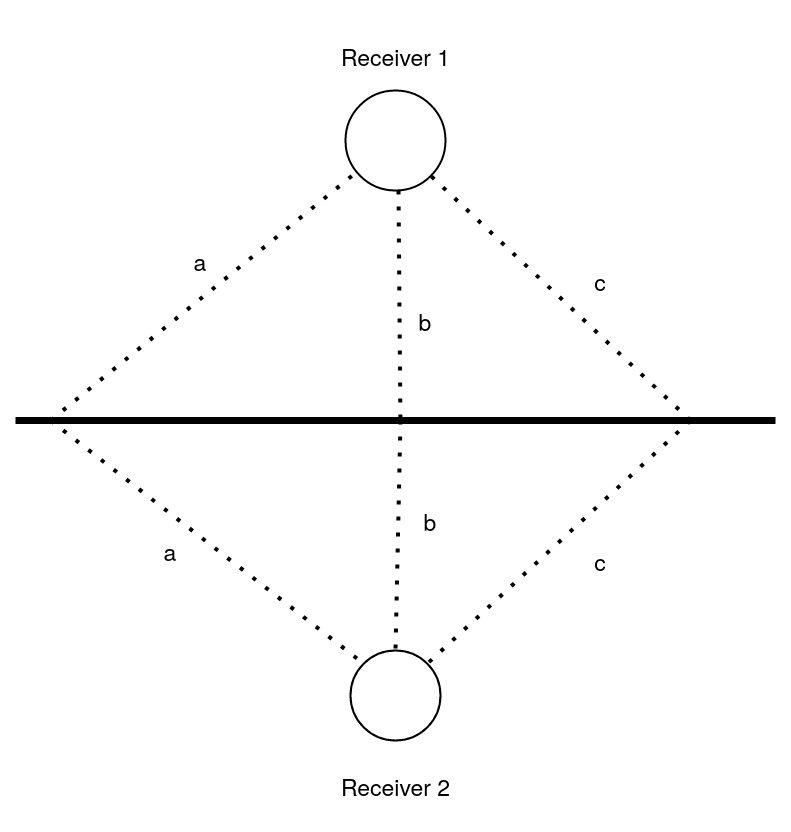
\includegraphics[width=0.6\linewidth]{../Photos/tdoa-dt-0.png}\\
      {(a) $Δt = 0$}
    \end{minipage}%
    % -----------------
    \begin{minipage}{.5\textwidth}
      \centering
      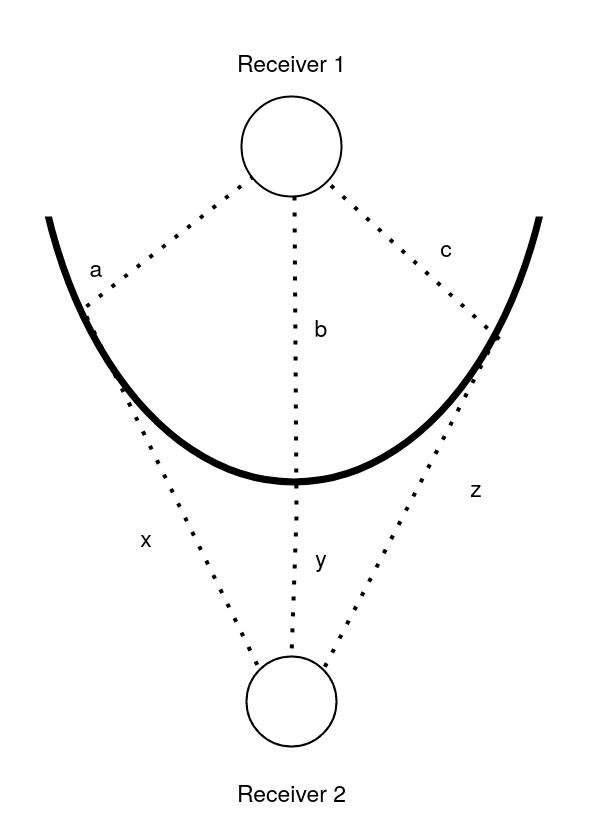
\includegraphics[width=0.4\linewidth]{../Photos/tdoa-dt-not-0.png}\\
      {(b) $Δt \neq 0$}
	\end{minipage}
	% -----------------
    \hfill \break
    \decoRule
    \caption[TDoA hyberbolas based on $\Delta t$]{TDoA hyberbolas based on $\Delta t$}
    \label{fig:TDoA-hyberbolas}
\end{figure}
\begin{align}
	\Delta t = a-a = 0 \quad \quad \quad & \quad \quad \quad\Delta t = x-a \nonumber \\
	\Delta t = b-b = 0 \quad \quad \quad & \quad \quad \quad\Delta t = y-b \nonumber \\
	\Delta t = c-c = 0 \quad \quad \quad & \quad \quad \quad\Delta t = z-c \nonumber
\end{align}


Η δεύτερη εκδοχή της χρήσης \Abbr{TDoA} - η οποία είναι πιο συχνή στα \Abbr{WSN} και 
μας ε\-νδια\-φέ\-ρει περισσότερο, 
χρησιμοποιεί multiple signals με single receiver και παρουσιάζεται στην \Fig{Time-Difference-of-Arrival-cases} (b). 
Αρχή λειτουργίας έχει ότι ο transmitter θα στείλει πολλαπλά - διαφορετικού είδους - σήματα και ο δέκτης θα μετρήσει την χρονική διαφορά 
που τα έλαβε. Ως παράδειγμα μπορεί το ένα σήμα να είναι σε \Abbr{RF} και να κινείται με ταχύτητα $s_r=c_o$ και το άλλο 
ηχητικό με ταχύτητα $s_s \approx 343m/s$ \footnote{Για μετάδοση σε ξηρό αέρα υπό θερμοκρασία \SI{20}{\celsius} \cite{wikipedia-speed-of-sound}}. 
Αν $t_r$ η χρονική στιγμή που λαμβάνει το \Abbr{RF} σήμα, $t_s$ το ηχητικό και $t_d$ το delay που μεσολάβησε από την αποστολή του ενός στο άλλο,
τότε μπορούμε να υπολογίσουμε την απόσταση μεταξύ των κόμβων από την εξίσωση \EqNum{tdoa-distance}
\cite{wsn-Localization-systems} \cite{localization-algorithms}.

\begin{align}
	d=&(s_r-s_s)(t_s-t_r-t_{d}) \label{eq:tdoa-distance}
\end{align}

Θετικό σε αυτήν την μέθοδο είναι ότι το error μπορεί να είναι της τάξης των μερικών εκατοστών, όμως αρχικά απαιτεί επιπλέον εξοπλισμό στο node -
ώστε να μπορεί να στείλει και να λάβει πολλαπλά είδη σήματος - πράγμα που μπορεί να το κάνει αντι\-οι\-κο\-νο\-μι\-κό ή αρκετά μεγαλύτερο σε διαστάσεις από 
το επιθυμητό. Όπως επίσης - και μάλιστα  
σημαντικότερο - η απόσταση η οποία μπορεί να 
χρησιμοποιηθεί, επηρεάζεται σε μεγάλο βαθμό από τα χαρακτηριστικά του δεύτερου σήματος. Ως παράδειγμα, τα ηχητικά σήματα 
δεν μπορούν να μεταφερθούν σε μεγάλες αποστάσεις ή το ότι η ταχύτητα τους μπορεί να επηρεαστεί σημαντικά από περιβαλλοντολογικούς παράγοντες
\cite{farooqiazam2016location}.\footnote{Η συγκεκριμένη μέθοδος είναι διαισθητικά παρόμοια, με αυτό που θα κάναμε για να εκτιμήσουμε 
την απόσταση μίας αστραπής από εμάς, μετρώντας το χρονικό διάστημα μέχρι να ακούσουμε την βροντή.} 

%----------------------------------------------------------------------
\subsubsection{Angle}\label{sec:Chapter3-1-2}

Άλλη μία χρήσιμη μέτρηση η οποία μας ενδιαφέρει, είναι η εκτίμηση της γωνίας από την οποία λαμβάνουμε το σήμα ενός γειτονικού
node σε σχέση με έναν άξονας αναφοράς. Ο άξονας αυτός μπορεί να είναι είτε κοινώς για όλα τα nodes (π.χ. ως προς το βόρειο γεωγραφικό πόλο),
είτε μπορεί να είναι για το κάθε node ξεχωριστός, ως παράδειγμα με βάση τον προσανατολισμό του ίδιου του node ή με βάση την γωνία λήψης ενός 
επιπλέον σήματος \cite{wsn-Localization-systems}. Την πληροφορία αυτή την βρίσκουμε στην βιβλιογραφία να ονομάζεται Angle of Arrival 
(\Abbr{AoA}) ή Direction of Arrival (\Abbr{DoA}). 

\begin{align}
	s(t)=A\sin(2\pi ft + \phi) \label{eq:signal-equation}
\end{align}

Γνωρίζουμε ότι ένα σήμα καθορίζεται πλήρως από τρεις παραμέτρους, το πλάτος του A, την συχνότητα του \emph{f} καθώς 
επίσης και από την φάση του $\phi$ - σχέση \EqNum{signal-equation}. Για τον υπολογισμό της γωνίας \Abbr{AoA} μπορούν 
να χρησιμοποιηθούν τεχνικές με γνώμονα τα παραπάνω. 

\subsubsection{Amplitude response}
Ο όρος \emph{Beamforming} \cite{wikipedia-beamforming} χρησιμοποιείται για να περιγράψει το pattern 
της ευαισθησίας του σήματος που στέλνει/λαμβάνει μία \emph{directional antenna} \cite{wikipedia-directionl-antenna}. 
% ή γενικά στην χρήση του μοντέλου της \emph{anisotropy antenna}. 
Το pattern αυτού του τύπου κε\-ραί\-ας, παρουσιάζεται στην \Fig{Typical-anisotropic-antenna-pattern}
\cite{wsn-Localization-techniques} και μπορούμε να χρησιμοποιήσουμε αυτό το χαρακτηριστικό για τον υπολογισμό της \Abbr{AoA}. 
Εάν χρησιμοποιούμε \emph{directional ante\-nna} στον receiver και μπορούμε είτε με μηχανικό είτε με ηλεκτρονικό τρόπο να στρέψουμε
την κεραία σε διάφορες κατευθύνσεις, τότε μπορούμε μετρώντας το πλάτος του σήματος που λαμβάνουμε, να εκτιμήσουμε και την κατεύθυνση του - όπου ιδανικά
βρίσκεται εκεί από όπου έχουμε την μέγιστη τιμή του amplitude του κύματος. Σημαντικές παράμετροι για την εκτίμηση της γωνίας σε αυτήν την περίπτωση, 
είναι επίσης η ευαισθησία του δέκτη καθώς και το width του beam της. 
Λανθασμένη εκτίμηση μπορεί να προκύψει, αν για κάποιο λόγο το πλάτος του σήματος που λαμβάνουμε δεν είναι σταθερό. Σε αυτή την περίπτωση, μία λύση
είναι να χρησιμοποιήσουμε μία δεύτερη - μη κινούμενη - \emph{omnidirectional} κεραία και να κανονικοποιήσουμε τις μετρήσεις της \emph{directional} με βάση τις   
μετρήσεις της δεύτερης \cite{wsn-Localization-techniques}.

% IMAGE
\FigCaptLabelBasedURL{../Images/Theoretical-Background/A-typical-radiation-pattern-of-the-directive-antenna.jpeg}%	Image Path
{Typical anisotropic antenna pattern}%	Caption Text
{Typical-anisotropic-antenna-pattern}%	Label used
<0.3>% Scale of image
[wsn-Localization-techniques]%	Based on specific paper 
(https://www.sciencedirect.com/science/article/abs/pii/S1389128606003227) % URL that found

\subsubsection{Phase response}
Άλλος τρόπος υπολογισμού του \Abbr{AoA} είναι με την αξιοποίηση της πληροφορία για την φάση που έχουμε για ένα σήμα. Σε αυτήν την περίπτωση
χρειαζόμαστε ή κεραίες αρκετά μεγαλύτερες από το μήκος κύματος του σήματος που στέλνουμε, ή antenna arrays \cite{wsn-Localization-techniques}. 

Για τα κύματα γνωρίζουμε ότι η διαφορά φάσης $\Delta \phi$ δύο σημείων που απέχουν  
μεταξύ τους $\Delta \chi$ μπορεί να υπολογιστεί από την σχέση \EqNum{phase-different-general} \cite{phase-difference}.

\begin{align}
	\Delta \phi = 2\pi\frac{\Delta \chi}{\lambda} = 2\pi\frac{\Delta t}{T} \label{eq:phase-different-general}
\end{align}

Συνεπώς, αν σχεδιάσουμε ένα antenna array, όπου η κάθε κεραία απέχει από την γειτονική της σε συγκεκριμένη απόσταση \emph{d} και μετρώντας 
το phase difference του σήματος που λαμβάνουμε μεταξύ τους, τότε μπορούμε να υπολογίσουμε την γωνία πρόσληψης της ακτινοβολίας μέσω της 
σχέσης \EqNum{aoa-equation} \cite{wsn-Localization-techniques} \cite{youtube-phase-difference-equation}. Παράδειγμα αυτού\udot βρίσκεται στην \Fig{Antenna-Arrays} (a).
Σε αυτήν την περίπτωση χρησιμοποιούμε \emph{omnidirectional} κεραίες και o υπολογισμός της διαφοράς φάσης μπορεί να γίνει
μέσω μετρήσεων \Abbr{TDoA}.

\begin{gather} 
	\phi = \frac{2\pi}{\lambda}d\sin(\theta) \Rightarrow \nonumber \\[2pt]
	\theta = \sin^{-1}\left(\frac{\lambda \phi}{2\pi d}\right) \label{eq:aoa-equation}
\end{gather}

Δεν υπάρχουν όμως μόνο τα linear antenna arrays, μπορούμε να τα σχεδιάσουμε σε διάφορες διατάξεις, 
παράδειγμα μίας εξ' αυτών βρίσκεται στην \Fig{Antenna-Arrays} (b).

\begin{figure} [H]
	\centering
	% -----------------
    \begin{minipage}{.5\textwidth}
      \centering
      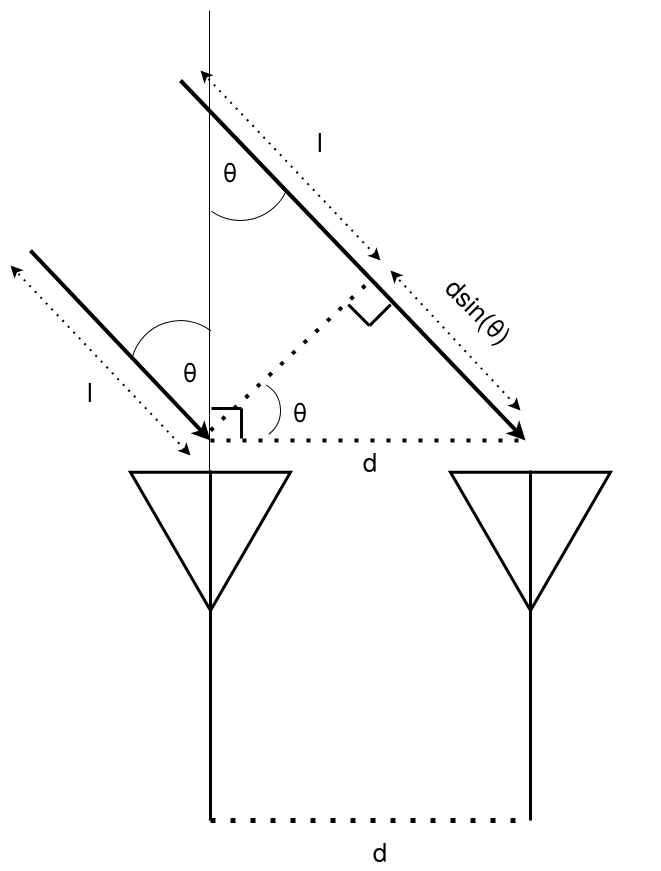
\includegraphics[width=0.5\linewidth]{../Photos/aoa-2antennas.png}\\
      {(a) Linear Two Antenna Array}
    \end{minipage}%
    % -----------------
    \begin{minipage}{.5\textwidth}
      \centering
      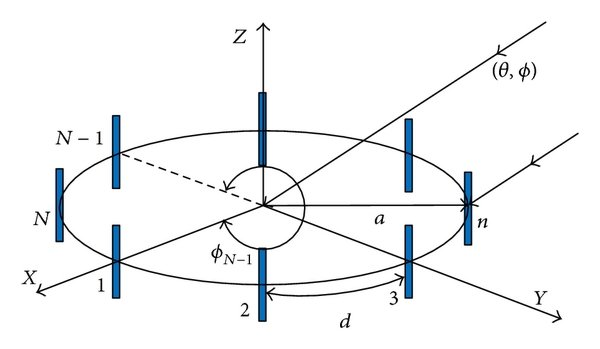
\includegraphics[width=.7\linewidth]{../Images/Theoretical-Background/The-antenna-array-geometry-a-linear-and-b-circular_W640.jpeg}\\
      {(b) Circular Antenna Array \URI{https://www.researchgate.net/publication/298331796_Adaptive_Array_Beamforming_Using_a_Chaotic_Beamforming_Algorithm/figures}}
	\end{minipage}
	% -----------------
    \hfill \break
    \decoRule
    \caption[Antenna Arrays examples]{Antenna Arrays examples}
    \label{fig:Antenna-Arrays}
\end{figure}

Η μέθοδος με την αξιοποίηση της σχέσης \EqNum{aoa-equation} λειτουργεί αρκετά καλά όταν έχουμε υψηλό Signal to Noise Ratio (\Abbr{SNR}),
αλλά μπορεί να έχει λανθασμένα αποτελέσματα όταν έχουμε διασυμβολικές παρεμβολές ή multipath signals. 
Επειδή στην πράξη εμφα\-νί\-ζονται και τα δύο, υπάρχει αρκετά μεγάλο επιστημονικό ενδιαφέρον να αντι\-με\-τω\-πι\-στεί αυτός ο περιορισμός.
Αρκετές τεχνικές έχουν προταθεί οι οποίες στρέφονται γύρω από την λογική του Maximum Likelihood (\Abbr{ML})
για τον υπολογισμό τελικά της γωνίας \cite{wsn-Localization-techniques}.

%----------------------------------------------------------------------------------------
%	SECTION 2
%----------------------------------------------------------------------------------------
\subsection{Position Computation} \label{sec:Chapter3-2} 
Αν έχουμε δύο nodes, οι μετρήσεις που λάβαμε από το \Sect{Distance-Angle-Estimation} είναι αρκετές για να γνωρίζουμε την θέση του καθενός,
συνεπώς ενδιαφέρον βρίσκεται στην ύπαρξη τριών ή παραπάνω nodes σε ένα σύστημα. Με βάση τις πληροφορίες που έχουμε συλλέξει - μέσω των τεχνικών που 
περιγράφτηκαν στο προηγούμενο κεφάλαιο - θα προσπαθήσουμε πλέον να εκτιμήσουμε την θέση ενός node. Στην συνέχεια αυτού του section, περιγράφονται μέθοδοι οι οποίοι μπορούν να χρησιμοποιηθούν για να το επιτύχουν
αυτό. Κύρια διαφορά τους είναι η απόδοση που μπορεί να έχουν, η οποία όμως σχετίζεται με την αύξηση της πολυπλοκότητας στους υπολογισμούς που θα
χρειαστούν\udot καθώς επίσης και ποιες από τις παραπάνω πληροφορίες θα εκμεταλλευτούν. 

Για την εύρεση της θέσης ενός unknown node στο τρισδιάστατο χώρο $(\mathfrak{R}^3)$ το Minimal Required number of Sensors (\Abbr{MRS}) είναι τέσσερα nodes.
Στις παρακάτω περιγραφές όμως, και χωρίς βλάβη της γενικότητας θα χρησιμοποιηθούν τρία για την απλούστευση της περιγραφής - με απώτερο σκοπό την εύκολη κατανόηση της, με την παραδοχή ότι μας
ενδιαφέρει η δισδιάστατη ανάλυση $(\mathfrak{R}^2)$. Ενώ στο \Chap{Chapter4} στο οποίο γίνεται και ο σχεδιασμός του συστήματος - βάση συγκεκριμένου αλγόριθμου - 
θα γίνει η ανάλυση στους τρεις άξονες.

%----------------------------------------------------------------------
\subsubsection{Trilateration}
Η συγκεκριμένη μέθοδος είναι ίσως η πιο απλή διαισθητικά, βασίζεται στην γεωμετρία κύκλων, είναι αυτή που χρησιμοποιείται από τα \Abbr{GPS}
για τον υπολογισμό θέσης \cite{trilateration-vs-triangulation-video}, ενώ αξιοποιεί μόνο πληροφορία απόστασης και όχι γωνίας \cite{Trilateration-vs-Triangulation}.
Η εξίσωση ενός κύκλου από την γεωμετρία γνωρίζουμε ότι περιγράφεται από την εξίσωση \EqNum{trilateration-circles} όπου $(x_i,y_i)$ οι συντεταγμένες
του κέντρο του κύκλου με ακτίνα $r_i$.

\begin{align}
	(x-x_i)^2 + (y-y_i)^2 &= r_i^2 \label{eq:trilateration-circles}
\end{align}

\begin{figure} [H]
	\centering
    % -----------------
		\begin{minipage}{.5\textwidth}
			\centering
			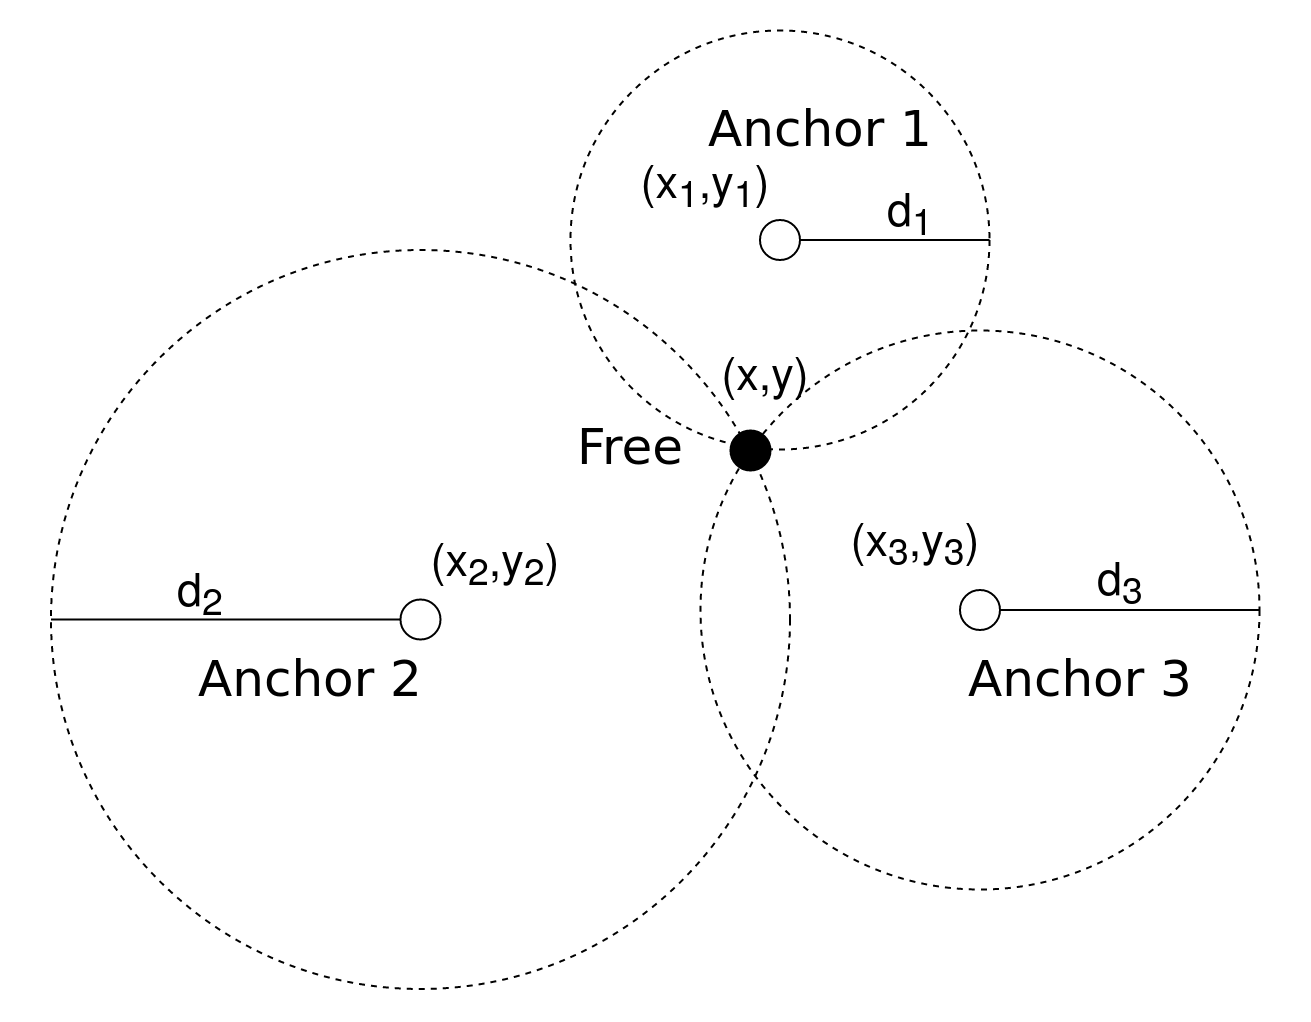
\includegraphics[width=0.7\linewidth]{../Photos/Trilateration-ideal.png}\\
			{(a) Ideal Trilateration}
		\end{minipage}%
		% -----------------
		\begin{minipage}{.5\textwidth}
			\centering
			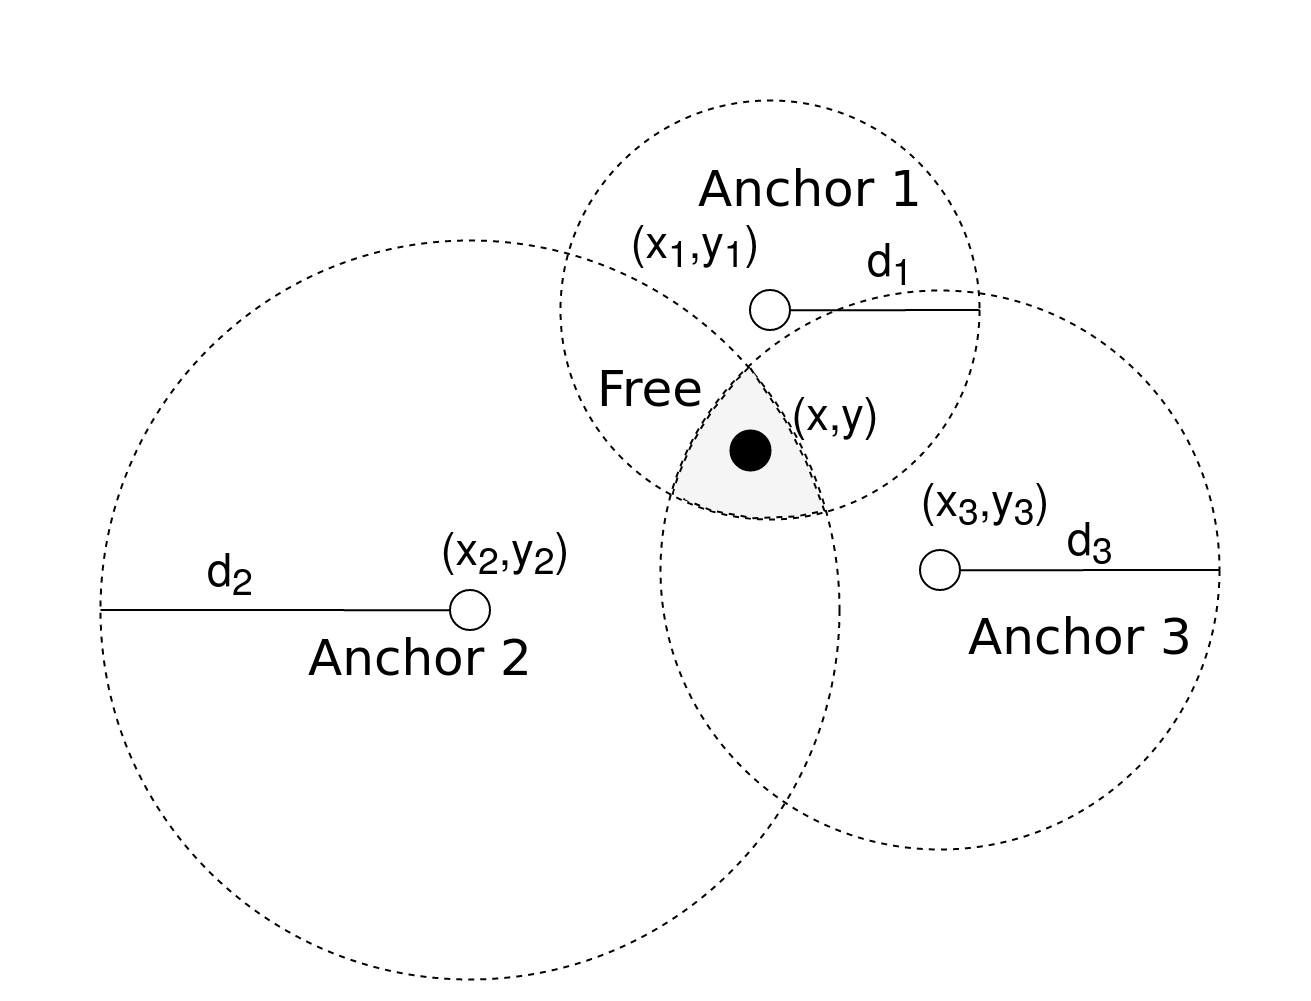
\includegraphics[width=.7\linewidth]{../Photos/Trilateration-actual.png}\\
			{(b) Realistic Trilateration}
		\end{minipage}
	% -----------------
    \hfill \break
    \decoRule
    \caption[Trilateration examples]{Trilateration examples}
    \label{fig:Trilateration-examples}
\end{figure}

Εάν χρησιμοποιούμε \emph{omnidirectional κεραίες} \cite{Omnidirectional-antenna} ή στην γενικότερη περίπτωση το μοντέλο της \emph{isotropic antenna} \cite{Isotropic-radiator} και υπολογίσουμε την απόσταση ενός beacon από το node στο οποίο θέλουμε να υπολογίσουμε την θέση του -
τότε μπορούμε να συμπεράνουμε ότι το free node είναι κάπου πάνω στην περιφέρεια ενός 
κύκλου, με κέντρο το beacon και ακτίνα την απόσταση μεταξύ του beacon και του free node. 
Επαναλαμβάνοντας αυτό για ακόμα δύο beacons, τελικά το free node στο δισδιάστατο επίπεδο $(\mathfrak{R}^2)$ θα πρέπει να βρίσκεται στην τομή των τριών κύκλων, πράγμα που γραφικά 
απεικονίζεται στην \Fig{Trilateration-examples} (a) \cite{RSSI-trilateration-Range_based}.

\begin{align}
	x^2-2 x_1 x + x_1^2 + y^2-2 y_1 y + y_1^2 &= r_1^2 \label{eq:trilateration-b1} \\ 
	x^2-2 x_2 x + x_2^2 + y^2-2 y_2 y + y_2^2 &= r_2^2 \label{eq:trilateration-b2} \\
	x^2-2 x_3 x + x_3^2 + y^2-2 y_3 y + y_3^2 &= r_3^2 \label{eq:trilateration-b3} 
\end{align}

Οι εξισώσεις \EqNum{trilateration-b1}, \EqNum{trilateration-b2} και \EqNum{trilateration-b3} περιγράφουν πλήρως τους κύκλους του κάθε node από το παράδειγμα 
του \Fig{Trilateration-examples} (a),
όπου $(x_i,y_i)$ το κέντρο του κύκλου, $r_i$ η ακτίνα του - για κάθε beacon $i=1,2,3$ και τελικά $(x,y)$ οι συντεταγμένες του free nodes τις οποίες και ψάχνουμε. 
Ένας τρόπος να υπολογίσουμε τις συντεταγμένες αυτές είναι να αφαιρέσουμε από την \EqNum{trilateration-b2} την \EqNum{trilateration-b1} και όμοια από την 
\EqNum{trilateration-b3} την \EqNum{trilateration-b2} ώστε να καταλήξουμε στις παρακάτω δύο εξισώσεις \cite{trilateration-equations} \cite{localization-algorithms-for-wsn}.

\begin{align}
	(-2x_1+2x_2)x + (-2y_1+2y_2)y = r_1^2 - r_2^2 - x_1^2 + x_2^2 - y_1^2 + y_2^2  \nonumber \\
	(-2x_2+2x_3)x + (-2y_2+2y_3)y = r_2^2 - r_3^2 - x_2^2 + x_3^2 - y_2^2 + y_3^2  \nonumber
\end{align}

Ο λόγος που κάναμε το παραπάνω βήμα είναι διότι πλέον έχουμε ένα σύστημα με δύο εξισώσεις και δύο αγνώστους, οπότε μπορούμε εύκολα να θεωρήσουμε τους παρακάτω πίνακες.

\begin{align}
	A = \begin{bmatrix} -2x_1+2x_2 & -2y_1+2y_2 \\ -2x_2+2x_3 & -2y_2+2y_3 \end{bmatrix} \nonumber \quad
	X = \begin{bmatrix} x \\ y \end{bmatrix} \nonumber \quad
	B = \begin{bmatrix} r_1^2 - r_2^2 - x_1^2 + x_2^2 - y_1^2 + y_2^2 \\ r_2^2 - r_3^2 - x_2^2 + x_3^2 - y_2^2 + y_3^2 \end{bmatrix} \nonumber
\end{align}

Με την χρήση των οποίων καταλήγουμε ότι έχουμε να λύσουμε το γραμμικό σύστημα πινάκων που περιγράφεται από την εξίσωση \EqNum{trilateration-linear-system} για τον
υπολογισμό των συντεταγμένων $(x,y)$ του free node οι οποίες μας ενδιαφέρουν.

\begin{align}
	AX = B \label{eq:trilateration-linear-system}
\end{align}

Όπως αναφέρθηκε και στις προηγούμενες ενότητες, ο υπολογισμός της απόστασης πολύ πιθανόν να περιλαμβάνει μια μικρή απόκλιση $\widehat{r_i} = r_i - ε$, 
με το ε συχνά να θεωρείται μία ανεξάρτητη κανονική τυχαία μεταβλητή με μηδενικό μέσο. Αυτό σημαίνει ότι
τότε οι κύκλοι δεν έχουν ένα κοινό σημείο τομής, αλλά το free node βρίσκεται κάπου μέσα στο χωρίο επικάλυψης
των τριών κύκλων, σχηματικά αυτό παρουσιάζεται στην \Fig{Trilateration-examples} (b) και σε αυτήν την περίπτωση καταλήγουμε σε ένα
μη πεπερασμένο πλήθος λύσεων, με τη συνάρτηση του κάθε κύκλου να περιγράφεται από την εξίσωση
\EqNum{trilateration-circles-error} \cite{wsn-Localization-systems}.

\begin{align}
	(x-x_i)^2 + (y-y_i)^2 &= r_i^2-e \label{eq:trilateration-circles-error}
\end{align}

Το αρνητικό με αυτήν την μέθοδο, είναι η ανάγκη πραγματοποίησης floating point operations για τον υπολογισμό των συντεταγμένων $(x,y)$ σε πραγματικές συνθήκες - όπου το πλήθος
των οποίων εξαρτάται από τον τρόπο που θα επιλέξουμε να επιλύσουμε το σύστημα. 
Μία από τις μεθόδους επίλυσης της γραμμικής εξίσωσης είναι μέσω του least square method, όπου τότε το πλήθος των floating point operations
που απαιτούνται είναι $(m+\frac{n}{3})\cdot n^2$, με $m$ τον αριθμό των αγνώστων και $n$ τον αριθμό των δοθέντων εξισώσεων \cite{wsn-Localization-systems}.

%----------------------------------------------------------------------
\subsubsection{Bounding Box}
Σε αυτήν την μέθοδο χρησιμοποιούνται τετράγωνα αντί για κύκλους του Tri\-la\-te\-ra\-tion, ενώ και εδώ θεωρούμε $(x_i,y_i)$
τις συντεταγμένες των beacon και $d_i$ η από\-στα\-ση που έχουμε υπολογίσει από το free node - για κάθε beacon $i$. 

% IMAGE
\FigCaptLabelBasedURL{../Photos/Bounding-box.png}%
{Bounding Box example}%
{Bounding-Box-example}%
<0.4>

Δημιουργούμε
τετράγωνα μήκος πλευράς $2d_i$ με κέντρο το κέντρο του beacon και συντεταγμένες $(x_i - d_i, y_i - d_i)$ \& $(x_i + d_i, y_i + d_i)$. 
Θετικό πλέον είναι ότι δεν χρειάζεται να κάνουμε floating point operations για τον υπολογισμό του χωρίου τομής - αλλά μπορούμε να το υπολογίσουμε
με απλή γεωμετρία. Αφού έχουμε υπολογίσει το χωρίο τομής των τετραγώνων μπορούμε να θεωρήσουμε ότι στο κέντρο του βρίσκεται το free node.
Παράδειγμα αυτής της μεθόδου βρίσκεται στην \Fig{Bounding-Box-example}.
Η συγκεκριμένη μέθοδος μπορεί να είναι ευκολότερη υπολογιστικά και να απαιτεί λιγότερα processor resources από το Trilateration, όμως ταυτόχρονα 
προκύπτει και μεγαλύτερο σφάλμα απόκλισης \cite{wsn-Localization-systems}.   


%----------------------------------------------------------------------
\subsubsection{Triangulation}
Σε αντίθεση με τις παραπάνω μεθόδους, η τεχνική Triangulation εκτιμάει την θέση του node που μας ενδιαφέρει, χρησιμοποιώντας   
γνώση που έχουμε για γωνίες και όχι εκτίμηση της απόστασης. Ένα απλούστερο παράδειγμα παρουσιάζεται στην \Fig{Principles-of-Triangulation}, όπου σε αυτό το παράδειγμα από την τριγωνομετρία,
μπορούμε εύκολα να συμπεράνουμε ότι για τις γωνίες $\theta_1$ και $\theta_2$ ισχύουν οι σχέσεις \EqNum{angle-equations-triangulation}.

% IMAGE
\FigCaptLabelBasedURL{../Photos/Tringulation-principle.png}%
{Principles of Triangulation}%
{Principles-of-Triangulation}%
<0.4>

\begin{align}
	\theta_1 = \frac{d}{d_1} = tan^{-1}\left(\frac{y_1-y}{x_1-x}\right) \quad \quad \quad
	\theta_2 = \frac{d}{d_2} = tan^{-1}\left(\frac{y_2-y}{x_2-x}\right) \label{eq:angle-equations-triangulation}
\end{align}

Από τις σχέσεις \EqNum{angle-equations-triangulation} μπορούμε να καταλήξουμε στις σχέσεις \EqNum{triangilation-principle} \cite{triangulation-simple-equation}, μέσω 
των οποίων τελικά για δεδομένες θέσεις των beacon - γνωστά δηλαδή τα $(x_i,y_i)$ για κάθε beacon i - και με βάση την μέτρηση των γωνιών $\theta_1$ και $\theta_2$,
να υπολογίσουμε την θέση του free node $(x,y)$.

\begin{equation}
	\begin{gathered}
		x = \frac{y_2 - y_1-  x_2\tan \theta_2 + x_1\tan \theta_1}{\tan \theta_1 - \tan \theta_2} \\[4pt]
		y = x\tan \theta_1 + y_1 - x_1\tan \theta_1 \quad = \quad x\tan \theta_2 + y_2 - x_2\tan \theta_2    
	\end{gathered}
	\label{eq:triangilation-principle}
\end{equation}

\begin{figure} [H]
	\centering
	\hspace*{+2cm}\begin{minipage}{0.4\textwidth}
		\centering
		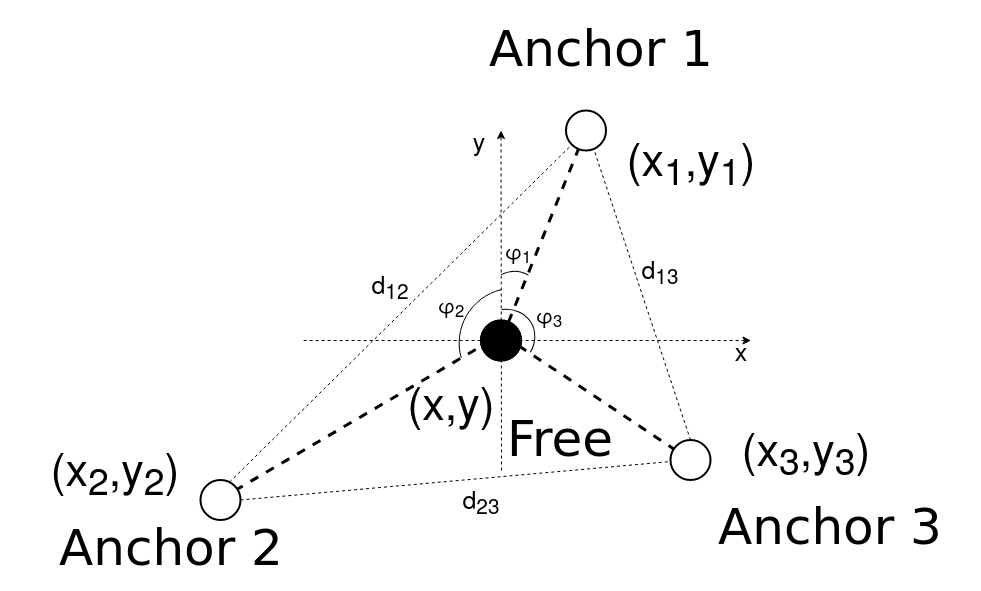
\includegraphics[width=0.8\linewidth]{../Photos/Tringulation-local.png}\\
		{(a) Local}
	\end{minipage}
	\newline
	\hspace*{+1cm}\begin{minipage}{.4\textwidth}
		\centering
		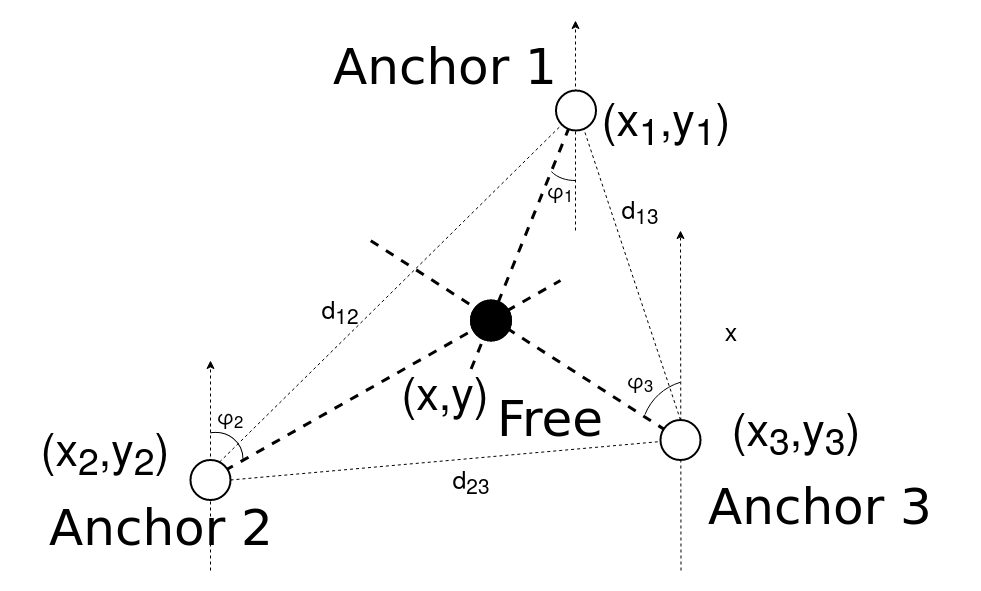
\includegraphics[width=.8\linewidth]{../Photos/Tringulation-remote.png}\\
		{(b) Remote Ideal}
	\end{minipage}%
	% -----------------
	\begin{minipage}{.4\textwidth}
		\centering
		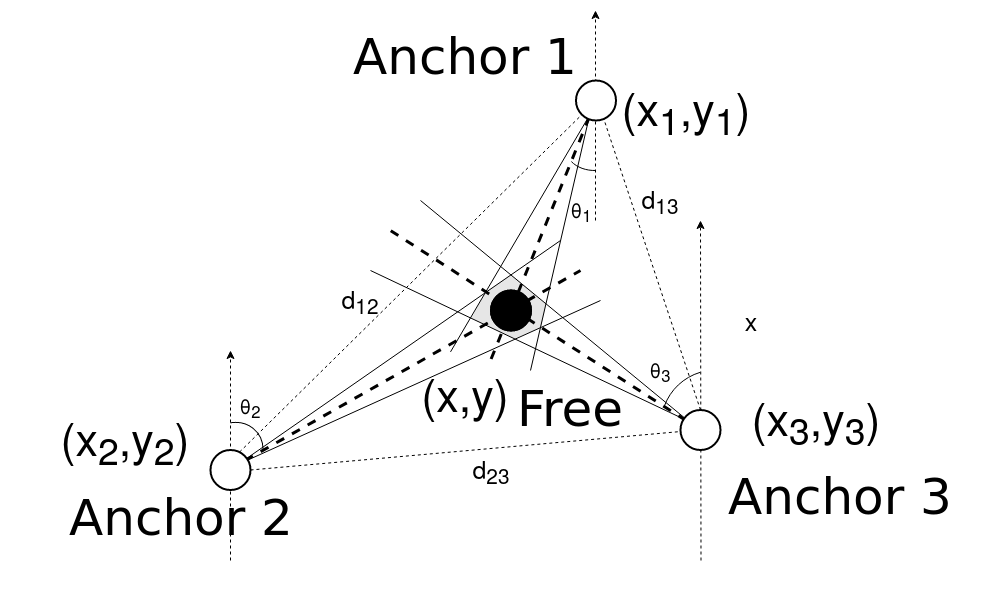
\includegraphics[width=.8\linewidth]{../Photos/Tringulation-remote-actual.png}\\
		{(c) Realistic}
	\end{minipage}
	\hfill \break \\
	\decoRule
	\caption[Triangulation examples]{Triangulation examples}
	\label{fig:Triangulation-examples}
\end{figure}

Αυτή η τεχνική εκτίμησης της θέσης του node, μπορεί να γίνει είτε από τοπικές μετρήσεις του ίδιου του node -
\Fig{Triangulation-examples} (a) - είτε από μετρήσεις γωνιών που κάνουν τα anchors - \Fig{Triangulation-examples} (b)
\cite{wsn-Localization-systems}. Φυσικά σε μία πραγματική εφαρμογή, όπως έχει αναφερθεί παραπάνω, οι μετρήσεις παρουσιάζουν αποκλίσεις 
από τα ιδανικά μοντέλα. Συνεπώς την \Fig{Triangulation-examples} (c) παρουσιάζει σε πιο ρεαλιστικά επίπεδα - συνυπολογίζοντας την ύπαρξη 
των αποκλίσεων - 
το χωρίο στο οποίο με μεγαλύτερη πιθανότητα βρίσκεται το node.

%----------------------------------------------------------------------
\subsubsection{Multilateration} \label{sec:Multilateration}
Η μέθοδος του Multilateration\footnote{Κάποιες φορές ο όρος αυτός χρησιμοποιείται επίσης σε αναφορά της χρήσης του Trilateration ή του Triangulation με πάνω από 3 beacons \cite{wsn-Localization-systems} \cite{triangulation-simple-equation}.} (\Abbr{MLAT}), 
έχει ως βάση την γεωμετρία των υπερβολικών καμπύλων και συχνά μπορεί να βρεθεί επίσης και ως hyperbolic positioning 
στην βιβλιογραφία \cite{multilateration-def} \cite{triangulation-trilateration-multilateration} \cite{wikipedia-multilateration}. στη \Sect{Distance-Angle-Estimation} 
έγινε αναφορά ότι η χρήση του \Abbr{TDoA} βασίζεται στις υπερβολικές καμπύλες, συνεπώς μπορούμε εύκολα να χρησιμοποιήσουμε
της μετρήσεις αυτές για τον υπολογισμό της θέσης του free node.

Η γενική ιδέα σε αυτήν την περίπτωση περιγράφεται στην εξίσωση \EqNum{tdoa-multiple} \cite{wsn-Localization-techniques} \cite{simple-tdoa} - και αυτό που 
θέλουμε, είναι να υπολογίσουμε την θέση του $k_t$ (free node) γνωρίζοντας για κάθε δύο διαφορετικά $k_i$ και $k_j$ beacon nodes
την χρονική στιγμή $t_i$ και $t_j$ που έφτασε το σήμα στο καθένα - εάν αυτό κινούταν με ταχύτητα s και το $\norm{\cdot}$ συμβολίζει την ευκλείδεια
απόσταση μεταξύ τους.

\begin{align}
	\Delta t_{ij} \triangleq & t_i - t_j = \frac{1}{s} (\norm{k_i - k_t} - \norm{k_j - k_t}), \quad i \neq j\label{eq:tdoa-multiple}
\end{align}

Αυτό που αναπαριστά ουσιαστικά η σχέση \EqNum{tdoa-multiple} δεν είναι τίποτα άλλο από την προσπάθεια εύρεσης του σημείου τομής των καμπύλων.
Παράδειγμα αυτής της μεθόδου βρίσκεται στην \Fig{Multilateration}.

% IMAGE
\FigCaptLabelBasedURL{../Photos/multilateration.png}%
{Multilateration example}%
{Multilateration}%
<0.4>

%----------------------------------------------------------------------
\subsubsection{Probabilistic approaches}
Το γεγονός ότι οι μετρήσεις απόστασης και γωνίας σε πραγματικές συνθήκες εμπε\-ριέ\-χουν σφάλματα, έχει ωθήσει στην έρευνα 
probabilistic μεθόδων εκτίμησης τοποθεσίας των free nodes. Αυτού του τύπου οι προσεγγίσεις λαμβάνουν υπόψιν τα μετρικά σφάλματα και συχνά τα μοντελοποιούν ως κανονικές
τυχαίες μεταβλητές. Το μεγάλο μειονέκτημα σε αυτήν την μέθοδο είναι τα μεγάλα υπολογιστικά και χωρικά - για την αποθήκευση των δεδομένων - κόστη \cite{wsn-Localization-systems}. 

\begin{table}[H]
    \caption[Distance/angle estimation techniques and position Computation summary]{Distance/angle estimation techniques and position Computation summary \cite{advantages-disadvantages-toa-tdoa-aoa}}
    \label{tab:Distance/angle-estimation-techniques-and-position-Computation-summary}
	\centering
	\resizebox{1\textwidth}{!}{
		\begin{tabular}{ccccc}
			\toprule
			\textbf{Method} & \textbf{Position Computetion}  & \textbf{Advantages} & \textbf{Disadvantages} & \textbf{Applications} \\
			\midrule
				\Abbr{RSSI} & 
					\*Pos*\ \Centerstack{Trila/Multilteration, \\ Bounding box} & 
					\*Adv*\ \Centerstack{Simple, inexpensive, \\no need for extra hardware, \\synchronization not needed} & 
					\*Dis*\ \Centerstack{Multipath interference, \\\Abbr{NLoS} and enviroment \\can affect readings} & 
					\*App*\ \Centerstack{In sort-distance with \Abbr{LoS} \\applications and low \\accuracy needed (e.g. indoor)} \\ \hline 
				\Abbr{ToA} & 
					\*Pos*\ \Centerstack{Trila/Multilteration, \\Bounding box} & 
					\*Adv*\ \Centerstack{High accuracy} & 
					\*Dis*\ \Centerstack{Need to precisely measure time, \\\Abbr{LoS} is normally assumed, \\more sophisticated design} & 
					\*App*\ \Centerstack{Common in cellular networks\\ or systems assisted by \Abbr{GPS}} \\ \hline
				\Abbr{TDoA} & 
					\*Pos*\ \Centerstack{Multilateration} & 
					\*Adv*\ \Centerstack{High accuracy} & 
					\*Dis*\ \Centerstack{Need for extra hardware \\or precisely synchronized nodes} & 
					\*App*\ \Centerstack{Common in \Abbr{WSN}\\ or systems assisted by \Abbr{GPS}} \\ \hline
				\Abbr{AoA} & 
					\*Pos*\ \Centerstack{Triangulation} & 
					\*Adv*\ \Centerstack{\Abbr{MRS} is two nodes (Ideal $\mathfrak{R}^2$), \\synchronization not needed} & 
					\*Dis*\ \Centerstack{\Abbr{LoS} is normally assumed, \\smart antenna design, \\multipath can affect readings} & 
					\*App*\ \Centerstack{Common in radar scenarios} \\ \hline
			\bottomrule
		\end{tabular}
	}
\end{table}

Στο \Tabl{Distance/angle-estimation-techniques-and-position-Computation-summary} γίνεται σύνοψη των μεθόδων εκτίμησης απόστασης
που αναλύθηκαν παραπάνω, μαζί με τις μεθόδους εκτίμησης θέσης που συχνά συνδυάζονται, καθώς και θετικά/αρνητικά όπως και συχνές τους εφαρμογές. 

%----------------------------------------------------------------------------------------
%	SECTION 3
%----------------------------------------------------------------------------------------
\subsection{Localization Algorithm} \label{sec:Chapter3-3} 
Στις προηγούμενες ενότητες αναφέρθηκαν κάποιες από τις βασικές τεχνικές που χρησιμοποιούνται, 
προκειμένου να εκτιμηθεί η θέση ενός node στον χώρο. Σε ένα πραγματικό σύστημα όμως, πρέπει να συνυπολογιστούν 
και άλλοι παράγοντες πέρα από - απλά - τον υπολογισμό απόστασης/γωνίας για να καταλήξουμε να αποκτήσουμε location information. 
Για αυτό το λόγο, στο παρόν \emph{Section} παρουσιάζονται επιπλέον πτυχές - του συστήματος - που πρέπει να λάβουμε 
υπόψιν\udot καθώς και αναφορά αλγό\-ρι\-θμων από την υπάρχουσα βιβλιογραφία, με τους οποίους μπορούμε να καλύψουμε αυτές τις
ανάγκες. 

Αφού έχουμε δει τα παραπάνω, αρχικά ας ορίσουμε το localization problem με ένα πιο αυστηρό μαθηματικό φορμαλισμό.
Έστω ότι έχουμε στην διάθεση μας \emph{n} αριθμό από nodes, και για λόγους απλότητας\udot συμμετρικά και όμοια δίκτυα
επικοινωνίας - με εμβέλεια \emph{r} - για κάθε node. Συνεπώς, ένα node \emph{u} επικοινωνεί με το \emph{v} αν και μόνο αν, και το
\emph{v} μπορεί να επικοινωνήσει πίσω στο \emph{u}, τα οποία είναι δια\-σκο\-ρπι\-σμένα σε ένα δισδιάστατο τετραγωνικό
πεδίο - και εδώ γίνεται η θεώρηση για $\mathfrak{R}^2$ ανάλυση - \emph{$Q=[0,s]\times[0,s]$}. 

Τότε μπορούμε να μοντελοποιήσουμε το δίκτυο από nodes, ως ένα μη κατευθυνόμενο γράφο $\mathcal{G} = (V, E)$ - παράδειγμα του οποίου υπάρχει στην \Fig{Graph-example} - με τα 
παρακάτω χαρακτηριστικά \cite{wsn-Localization-systems}.  

\begin{itemize}
	\item $V = \{v_1, v_2, ..., v_n\}$ το σύνολο των nodes, όπου έχει την έννοια των κορυφών του γράφου, με $|V| = n$\footnote{Ο 
	παραπάνω συμβολισμός $|\cdot|$ χρησιμοποιείται ως το cardinality του εκάστοτε set}.
	\item $\langle i,j\rangle \in E$ εάν το $u_i$ μπορεί να επικοινωνήσει με το $v_i$. Πράγμα που σημαίνει - με βάση τα παραπάνω - 
	ότι η ευκλείδεια απόσταση τους\udot είναι μικρότερη από \emph{r} και έχει την έννοια των ακμών του γράφου, με $|E| = m$\footnotemark[\value{footnote}].
	\item $0 \le w(e) \le r$ με $e = \langle i,j\rangle$, να είναι το βάρος της κάθε ακμής και να χρησιμοποιείται για την έννοια της απόστασης $d_{ij}$
	μεταξύ του node $u_i$ με το $v_i$.
\end{itemize}

% IMAGE
\FigCaptLabelBasedURL{../Photos/localization-graph.png}
{Graph example}%
{Graph-example}%
<0.4>

%----------------------------------------------------------------------
\subsubsection{One-hop vs Multi-hop}
Η πρώτη κατηγοριοποίηση στην οποία θα αναφερθούμε - για αυτό το δίκτυο γράφου - προκειμένου να εκτιμήσουμε την θέση των nodes, 
είναι από ποιους κόμβους τελικά θα αξιοποιήσουμε πληροφορία. Στους αλγόριθμους \textbf{One-hop} αξιοποιείται πληροφορία,
μόνο από άμεσους γείτονες των nodes\udot προκειμένου να υπολογίσουμε την θέση του κόμβου στο χώρο. Αντίθετα 
στις τεχνικές \textbf{Multi-hop}, χρησιμοποιούμε και πληροφορία που λαμβάνουμε με έμμεσο τρόπο\udot
από τους γείτονες των γειτόνων μας - προκειμένου να αποφανθούμε για την θέση ενός node.

%----------------------------------------------------------------------
\subsubsection{Anchor-based vs Anchor-free}
Ένας ακόμα σημαντικός διαχωρισμός είναι η ύπαρξη ή όχι τελικά στο δίκτυο - από anchor nodes. Καθώς υπάρχουν εφαρμογές
στις οποίες μπορεί να μην χρειάζεται ή να μην έχουμε δυνατότητα να τοποθετηθούν beacons - ακόμα και αν αναφερόμαστε σε mobile beacons -
οπότε τότε θα χρησιμοποιήσουμε \textbf{Anchor-free} αλγορίθμους. Αν υπάρχει η δυνατότητα χρήσης τους, τότε ενδιαφερόμαστε για
\textbf{Anchor-based}.

%----------------------------------------------------------------------
\subsubsection{Relative vs Absolute Positioning}
Ανάλογα με τις προδιαγραφές της εφαρμογής που θέλουμε να καλύψουμε, θα πρέπει να χρησιμοποιήσουμε ανάλογες εκτιμήσεις θέσεις.
Υπάρχουν εφαρμογές, όπως για παράδειγμα - εκτίμηση θέσεις των nodes ενός κινούμενου swarm\udot για χαρτογράφηση σε άγνωστο terrain. Σε αυτού 
του τύπου τις εφαρμογές μας ενδιαφέρει η απόλυτη θέση στον χώρο\udot οπότε θέλουμε μεθοδολογίες για \textbf{Absolute Positioning}, ενώ 
υπάρχουν άλλες εφαρμογές στις οποίες μας ενδιαφέρει μόνο πληροφορία θέσεις σε σχέση με τα υπόλοιπα στοιχεία του περιβάλλοντος της
εφαρμογής, οπότε χρειαζόμαστε \textbf{Relative Positioning}.

%----------------------------------------------------------------------
\subsubsection{Indoor vs Outdoor Scenarios}
Κάτι ακόμα που πρέπει να προσέξουμε είναι το περιβάλλον στο οποίο θα βρίσκεται η εφαρμογή, καθώς ανάλογα με το περιβάλλον\udot
έχουμε να διαχειριστούμε και τις δυσκολίες που μας παρουσιάζει - εμπόδια, ανακλάσεις σημάτων, κλπ. Με δύο κύριους διαχωρισμούς,
τα \textbf{Indoor Scenarios} και τα \textbf{Outdoor Scenarios}.

%----------------------------------------------------------------------
\subsubsection{Distributed vs Centralized Position Computation}
Πρέπει να αναφερθεί επίσης, ότι είναι πολύ σημαντικό να είναι ξεκάθαρο το σημείο\udot στο οποίο
θα γίνεται η επεξεργασία της πληροφορίας. Υπάρχουν δύο ενδεχόμενα. Το πρώτο
είναι, ένα \Abbr{BS} να αντιλαμβάνεται και να υπολογίζει την θέση των nodes, τα οποία
έπειτα θα ενημερώνονται μέσω αυτού\udot για την θέση τους - οπότε αναφερόμαστε για \textbf{Centralized} τεχνικές. Αντίθετα άλλη εναλλακτική 
είναι να γίνει τοπικά η επεξεργασία. Σε αυτή την περίπτωση, αναφερόμαστε για \textbf{Decentralized} ή \textbf{Distri\-bu\-ted} αλγορίθμους\udot όπου κάθε node θα 
επικοινωνεί από μόνο του με τα γειτονικά του για την απόκτηση πληροφορίας\udot και έπειτα υπολογίζει μεμονωμένα την θέση του. 
Το μεγάλο πλεονέκτημα των Centralized αλγορίθμων είναι ότι απομακρύνουμε το πρόβλημα του computation από το κάθε node, όμως την ίδια στιγμή
προκύπτουν δυσκολίες όπως καθυστερήσεις στις επικοινωνίες, μεγαλύτερο power consumption \& bandwidth, ενώ τέλος
και προβλήματα με το scalability του συστήματος - καθώς προτείνεται για μικρότερα networks. Το οποίο όμως σε ένα βαθμό\udot μπορεί να λυθεί
με το να χρησιμοποιηθούν πολλαπλά \Abbr{BS}s, συνεπώς να έχουμε ένα multi-tier network.
Γνωστοί Centralized αλγόριθμοι είναι o Multi Dimensional Scaling-Mobile Assisted Programming (\Abbr{MDS-MAP}), 
Semi Definite Programming (\Abbr{SDP}) και Localization Based on Simulated Annealing (\Abbr{LBSA}) \cite{range-distributed}.
Παρακάτω στον \Algo{MDS-MAP} - ως παράδειγμα
χρήσης των \emph{Centralized} αλγορίθμων - παρουσιάζεται ο pseudo-code του \Abbr{MDS-MAP}.

\begin{algorithm}[H]
	\caption[Multi Dimensional Scaling-Mobile Assisted Programming]{Multi Dimensional Scaling-Mobile Assisted Programming \cite{localization-algorithms}}\label{alg:MDS-MAP}
	\begin{algorithmic}[1]	% For line numbering just uncomment [1]
		\Statex{{\bf procedure} MDS-MAP ($r_{i,j} = w(e) \quad \forall \quad e \in E$)}
			\State Form a sparse matrix R from $r_{i,j}$
			\State Run a standard all pairs shortest path algorithm on R to produce \newline inter-node distances D (e.g. Dijkstra's, Floyd's)
			\State Run classical metric MDS on D to find estimated positions X
			\State Transform the solution X into global coordinates G
	\end{algorithmic}
\end{algorithm}

\begin{table}[H]
    \caption[Comparison of Centralized vs Distributed]{Comparison of Centralized vs Distributed \cite{localization-algorithms-comparizon-tables}}
	\label{tab:Comparison-of-Centralized-vs-Distributed}
	\centering
	\resizebox{0.7\textwidth}{!}{
		\begin{tabular}{lll}
			\toprule
			 & \textbf{Centralized} & \textbf{Distributed}\\
			\midrule
				Accuracy & Data collection & Position merging \\ 
				Energy consumption & Signal transition & Position merging \\ 
				Coverage area & Network topology & Anchor deployment \\ 
				Costs & Central module & Anchor equipment \\ 
			\bottomrule
		\end{tabular}
	}
\end{table}

% \begin{algorithm}[H]
% 	\caption{Localization Based on Simulated Annealing \cite{simulated-annealing} \cite{sal-localization}}\label{alg:LBSA}
% 	\begin{algorithmic}[1]
% 		\Statex{{\bf procedure} LBSA}($r_{i,j} = w(e) \quad \forall \quad e \in E$)
% 			\State Establishing an appropriate objective function $f(x)$
% 			\State Randomly and uniformly place nodes in a square region of side length L
% 	\end{algorithmic}
% \end{algorithm}

%----------------------------------------------------------------------
\subsubsection{Range-based vs Range-free}
στη \Sect{Energy-based} αναλύθηκαν τεχνικές εκτίμησης απόστασης ή γωνίας μεταξύ των nodes - συγκεκριμένα οι
\Abbr{RSSI}, \Abbr{ToA}, \Abbr{TDoA} και \Abbr{AoA}.
Σε αυτήν την περίπτωση, όταν χρησιμοποιούμε δηλαδή έξτρα hardware ή γενικά\udot εκτεταμένες ranging τεχνικές 
για να καταλήξουμε στις θέσεις των free nodes στον χώρο, αναφερόμαστε σε \textbf{Range-based} μεθόδους.
Θετικό σε αυτήν την περίπτωση είναι ότι έχουμε μεγαλύτερη ακρίβεια της θέσης, όμως ταυτόχρονα 
πιθανόν να χρειαστούμε ακριβότερα nodes - λόγο των έξτρα components ή του πιο \emph{sophisticated hardware}.  

Για να το αποφύγουμε αυτό, μπορούμε να χρησιμοποιήσουμε τεχνικές οι οποίες ονομάζονται \textbf{Range-free}. 
Αυτές οι τεχνικές δεν απαιτούν κανένα επιπρόσθετο hardware, διότι δεν χρησιμοποιούν εκτιμήσεις απόστασης/γωνίας, συνεπώς έχουμε μικρότερο κόστος ανά node. 
Έχουν αρκετό ενδιαφέρον λόγω της απλότητας τους\udot παρά την μικρότερη ακρίβεια που παρέχουν. Γνωστοί Range-free αλγόριθμοι είναι 
ο Approximate Point in Triangle (\Abbr{APIT}), 
Distance Vector-Hop (\Abbr{DV-Hop}), Centroid και Gradient \cite{range-distributed}.
Όμοια με παραπάνω, στους \Algo{APIT} και \ref{alg:DV-Hop} παρουσιάζονται οι pseudo-codes 
των \Abbr{APIT} και \Abbr{DV-Hop} αντίστοιχα.

% ALGORITHM
\begin{algorithm}[H]
	\caption[Approximate Point in Triangle]{Approximate Point in Triangle \cite{localization-algorithms}}\label{alg:APIT}
	\begin{algorithmic}[1]
			\Statex{{\bf procedure} APIT}
			\State Receive beacon positions from hear-able beacons.
			\State Initialize inside-set to be empty
			
			\For{each triangle $T_i$ in possible triangles formed over beacons}
				\State Add $T_i$ to inside-set if node is inside $T_i$.
					Go to next Step when accuracy
					\newline\hspace*{1.5em}of inside-set is sufficient.
			\EndFor
			
			\State Compute position estimate as the center of mass of the intersection of all 
			\newline triangles in inside-set.	
	\end{algorithmic}
\end{algorithm}

% ALGORITHM
\begin{algorithm}[H]
	\caption[Distance Vector-Hop]{Distance Vector-Hop \cite{dv-hop-algo} \cite{dv-hop-algo2} \cite{dv-hop-algo3}}\label{alg:DV-Hop}
	\begin{algorithmic}[1]
		\Statex{{\bf procedure} DV-Hop}{}
			
			\For{Each anchor}
				\State Broadcast a message with it's ID, location and hop count initialized to 0
      		\EndFor 
			
			\For{all nodes received all messages from neighbors}
				\State Neighbor nodes record the node ID, the coordinate values, and  the smallest  
				\newline\hspace*{1.5em}hop. Then forward packet after incrementing hop by one
      		\EndFor

			\For{each anchor i to each anchor j}
				\State Estimate Average Hop Distance (\Abbr{AHD}) \par
				\hspace*{7em}$HopSize_i = \frac{\sum{\sqrt{(x_i-x_j)^2+(y_i-y_j)^2}}}{\sum{hop_{i,j}}}, i\neq j$

				\State Broadcast \Abbr{AHD} to network
			\EndFor
			
			\For{each free node u}
				\State Save the first \Abbr{AHD} you hear, then broadcast it to your neighbors 
				\State Calculate your distance from your closest anchor \emph{k},
				$d_{uk} = HopSize_i \times hop_{uk}$
			\EndFor

			\State Based on known beacons' coordinates and estimated distances, use one of the methods described in 
			\Sect{Chapter3-2} to compute free nodes locations
	\end{algorithmic}
\end{algorithm}

% TABLE
\begin{table}[H]
    \caption[Comparison of Range-based vs Range-free]{Comparison of Range-based vs Range-free \cite{localization-algorithms-comparizon-tables}}
	\label{tab:Comparison-of-Range-based-vs-Range-free}
	\centering
	\resizebox{0.7\textwidth}{!}{
		\begin{tabular}{lll}
			\toprule
			 & \textbf{Range-based} & \textbf{Range-free}\\
			\midrule
				Accuracy & Ranging algorithm & Geometric algorithm \\ 
				Energy consumption & Signal transition & Instruction execution \\ 
				Coverage area & Signal cover & Network topology \\ 
				Costs & Ranging module & Execution module \\ 
			\bottomrule
		\end{tabular}
	}
\end{table}



% Horizontal Line
% \HLineWithSpaces<2>[300]<2>

Σε ευρύτερη κλίμακα, στην βιβλιογραφία υπάρχουν επιπλέον αλγόριθμοι ή παραλλαγές χρήσης αυτών που αναφέρθηκαν, για την εύρεση τοποθεσίας
nodes σε ένα \Abbr{WSN}. Παρόλα αυτά, σε αυτό το σημείο έγινε μία συνοπτική αναφορά τους,  και μία πρώτη
ανάλυση γύρω από το localization problem. Στην συνέχεια,
με βάση αυτές τις αρχές\udot θα γίνει η μοντελοποίηση του συστήματος που συσχετίζεται αυτή η διπλωματική. 

\newpage
% ----------------------------------------------------------------------------------------------------------------------------------------------------------
\section{Image-based Position Estimation} \label{chap:Image-based}
Άλλος ένας τρόπος για να καταλήξουμε να εκτιμήσουμε την θέση ενός αντικειμένου στον χώρο\udot είναι με την βοήθεια καμερών και οπτικών τεχνολογιών. Κύριος πε\-ριο\-ρι\-στι\-κός παράγοντας σε αυτές τις προσεγγίσεις, είναι η ανάγκη για οπτική επαφή με το αντικείμενο ενδιαφέροντος. Ενώ, καταλήγει να είναι και ο τρόπος με τις μεγαλύτερες ανάγκες επεξεργασίας. Βασικοί τρόποι απόκτησης \Abbr{3D} πληροφορίας - με χρήση \Abbr{2D}, που προσφέρει τυπικά μία κάμερα\footnote{Σε αντίθεση με τις RGB-D, οι οποίες εκτός από color information, παρέχουν και depth information για κάθε pixel τους} - είναι μέσω τεχνικών με όνομα structure from reference, structure from motion και με χρήση stereo \cite{location-from-image} οι οποίες συνοπτικά αναλύονται στην συνέχεια.

%----------------------------------------------------------------------
\subsection{Structure from Reference} \label{sec:theo-structure-from-reference}
Τυπικά, κατά τη μεταφορά των σημείων του πραγματικού κόσμου \Abbr{3D} σε pixel μίας εικόνας \Abbr{2D} χάνουμε την διάσταση του βάθους, πράγμα που μπορεί να δημιουργήσει πλάνες/αυταπάτες - παράδειγμα αυτού στην \Fig{depth-ambiguity-optical-illusion}. Ένας τρόπος για την επανάκτηση της πληροφορίας του depth - προκειμένου να εκτιμήσουμε μέσω εικόνας την θέση των αντικειμένων - είναι με το να υπάρχουν στο scene αντικείμενα γνωστών διαστάσεων, τα οποία θα χρησιμοποιηθούν ως reference objects.

\begin{figure} [H]
	\centering
    % -----------------
		\begin{minipage}{.4\textwidth}
			\centering
			\captionsetup{width=.9\linewidth}
			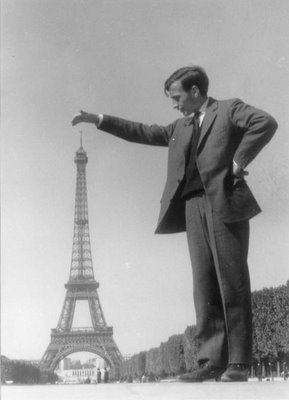
\includegraphics[width=0.8\linewidth]{../Images/Theoretical-Background/Two-well-known-optical-illusions-where-the-actual-depth-order-of-the-scene-objects-is.jpg}\\
			\decoRule
			\CaptionBasedwithURL{Optical illusion due to depth ambiguity of scene objects}%
			(https://www.researchgate.net/figure/Two-well-known-optical-illusions-where-the-actual-depth-order-of-the-scene-objects-is_fig4_285270806)
			\label{fig:depth-ambiguity-optical-illusion}
		\end{minipage}%
		% -----------------
		\begin{minipage}{.6\textwidth}
			\centering
			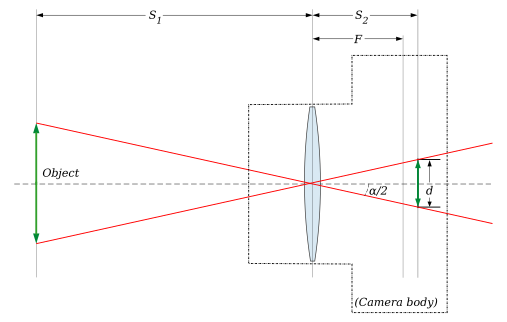
\includegraphics[width=\linewidth]{../Images/Theoretical-Background/Lens_angle_of_view.png}\\
			\decoRule
			\CaptionBasedwithURL{Optical axis from object to camera sensor}%
			(https://en.wikipedia.org/wiki/Angle\_of\_view) 
			\label{fig:optical-axis-from-object-to-camera-sensor}
		\end{minipage}
	% -----------------
    % \hfill \break
\end{figure}

Στην \Fig{optical-axis-from-object-to-camera-sensor} παρουσιάζονται οι νοητές ευθείες πορείας του φωτός στο thin lens model, από τα σημεία του τρισδιάστατου κόσμου, προς τον αισθητήρα της κάμερας. Όπου $S_1$ η απόσταση του αντικειμένου από την κάμερα σε $m$, $S_2$ η απόσταση του image plane για το pinhole model (περισσότερες πληροφορίες στη \Sect{design-implementation-camera}) σε $mm$, $F$ το focal length σε $mm$, $d$ το μέγεθος του αντικειμένου στην εικόνα σε $mm$ και $H$ το μέγεθος του αντικειμένου στον πραγματικό κόσμο σε $m$. Επίσης, θεωρούμε ότι το αντικείμενο είναι σε focus, συνεπώς $F=S_2$. Τότε, με χρήση τριγωνομετρίας και όμοιων τριγώνων τόσο από την μεριά του αισθητήρα, όσο και του αντικειμένου, καταλήγουμε στην σχέση \EqNum{distance-from-object-dim-triangles} \cite{calculate-distance-or-size-of-an-objectin-a-photo-image} \cite{calculate-distance-opencv} \cite{calculate-distance-stackexchange}.

\begin{align}
	\frac{d}{F} &= \frac{H}{S_1} \label{eq:distance-from-object-dim-triangles}
\end{align}

Από την οποία καταλήγουμε στο \Equa{distance-from-object}. Όπου στο μέγεθος του αντικειμένου μπορούμε να χρησιμοποιήσουμε οποιαδήποτε διάσταση επιθυμούμε, όπως το ύψος, το πλάτος ή ακόμα και κάποια διαγώνιο του.

\begin{align}
	\textrm{Distance to object $S_1$ (m)} &= \textrm{Focal length $F$ (mm)}\frac{\textrm{Object's real size $H$ (m)}}{\textrm{Object's size on sensor $d$ (mm)}} \label{eq:distance-from-object}
\end{align}

Σε γενικές γραμμές η αναδόμηση της τρίτης διάστασης από single view ακόμα και με ύπαρξη γνωστών αντικειμένων στο scene, μπορεί να καταλήξει να είναι μία εξαιρετικά ασαφής διαδικασία. Για αυτό τον λόγο προσπαθούμε είτε μέσω monocular vision να πάρουμε πολλαπλά views ενός κινούμενου αντικειμένου και να χρησιμοποιήσουμε τεχνικές με όνομα Structure from Motion (βλ. \Sect{theo-structure-from-motion}), είτε από πολλαπλές κάμερες - stereo vision (βλ. \Sect{theo-stereo}) - να λάβουμε πολλαπλά views στατικού αντικειμένου για την εκτίμηση τελικά του depth. 

%----------------------------------------------------------------------
\subsection{Structure from Motion} \label{sec:theo-structure-from-motion}
% IMAGE
\FigCaptLabelBasedURL{../Images/Theoretical-Background/sfm-exp.png}%
{Thesis drone swarm system overview}%
{thesis-system-overview}%
<0.7>%
(https://speciale.ar/publication/privacypreservingsfm/)



%----------------------------------------------------------------------
\subsection{Stereo Vision} \label{sec:theo-stereo}
Για τον υπολογισμό του depth με χρήση stereo vision, λαμβάνουμε από δύο κάμερες views ενός scene. Σε γενίκευση τα image planes μπορεί να έχουν οποιαδήποτε προσανατολισμό, ειδική περίπτωση - και συχνά πιο χρησιμοποιούμενη - είναι αυτή που υπάρχει στην \Fig{stereo-vision} (a) στην οποία είναι παράλληλα. Προκειμένου να εκτιμηθεί το depth με χρήση stereo γίνονται υπολογισμοί βασισμένοι στο Epipolar Geometry \cite{wiki-epipolar-geometry}.

\begin{figure} [H]
	\centering
    % -----------------
		\begin{minipage}{.5\textwidth}
			\centering
			% \captionsetup{width=.9\linewidth}
			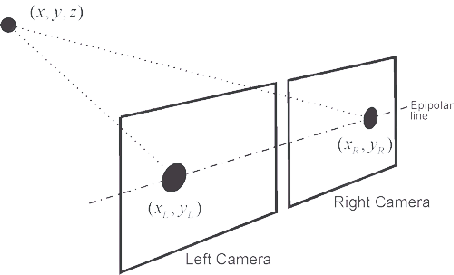
\includegraphics[width=\linewidth]{../Images/Theoretical-Background/Stereo-vision-principle.png}\\
			{(a) Stereo Vision Principle \URI{https://www.researchgate.net/figure/Stereo-vision-principle-two-cameras-which-view-the-same-scene-detect-a-common-3D-point_fig1_221908788}}
		\end{minipage}%
		% -----------------
		\begin{minipage}{.5\textwidth}
			\centering
			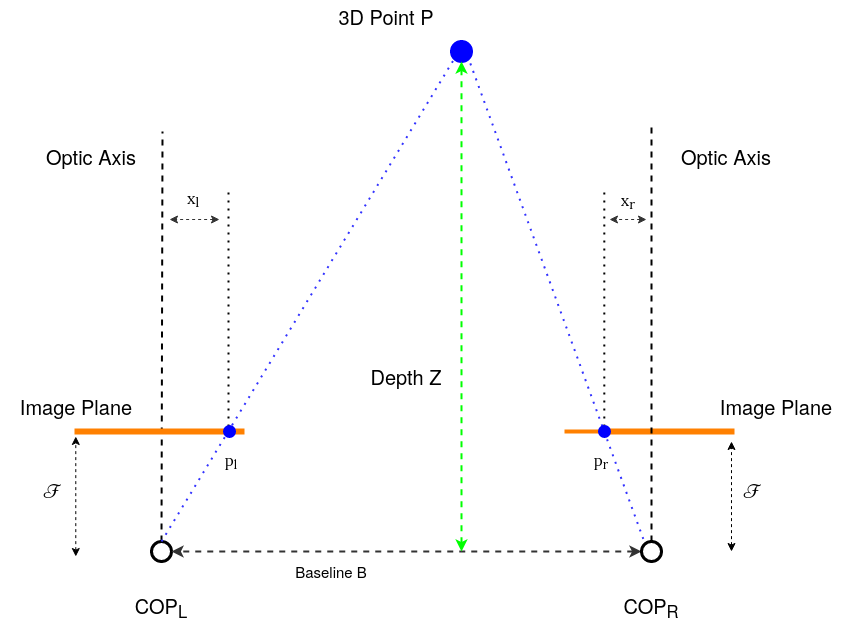
\includegraphics[width=\linewidth]{../Photos/stereo-math.png}\\
			{(b) Stereo Vision Geometry}
		\end{minipage}
	% -----------------
    \hfill \break \\
	\decoRule
	\caption[Stereo Vision]{Stereo Vision}
	\label{fig:stereo-vision}
\end{figure}

Η \Fig{stereo-vision} (b) παρουσιάζει την γεωμετρία στην περίπτωση των parallel optical axis. Μέσω σχέσεων των όμοιων τριγώνων $(p_l, P, p_r)$ και $(COP_L, P, COP_R)$ μπορούμε να δημιουργήσουμε την σχέση \EqNum{stereo-basic-eq}, από την οποία τελικά καταλήγουμε στο \Equa{stereo-depth-est} για τον υπολογισμό του depth ενός Point \cite{introduction-to-computer-vision}. 

\begin{gather}
	\frac{B-x_l+x_r}{Z-F} = \frac{B}{Z} \Rightarrow \label{eq:stereo-basic-eq} \\
	Z = F \frac{B}{x_l - x_r} \label{eq:stereo-depth-est}
\end{gather}

Η ποσότητα $x_l - x_r$ ονομάζεται Disparity, και ουσιαστικά μετρώντας την διαφορά της θέσης που εμφανίζεται στο κάθε plane το point, υπολογίζουμε την απόσταση του σημείου από το baseline των καμερών \cite{introduction-to-computer-vision}.

% This should be the last section
\section{Thesis Approach} \label{chap:thesis-approach}
Σκοπός της παραπάνω βιβλιογραφικής αναζήτησης\udot ήταν η απόκτηση μίας σφαιρικής γνώσης σχετικά με τους δυνατούς τρόπους επίλυσης του προβλήματος εντοπισμού της θέσης αντικειμένων, ώστε να πραγματοποιηθεί μία αρχική εκτίμηση της πολυπλοκότητας και του κόστους hardware που απαιτεί η κάθε μία, προκειμένου τελικά να γίνει η επιλογή της μεθοδολογίας με την οποία θα υλοποιηθεί στην συγκεκριμένη εργασία\udot η επίλυση του προβλήματος ενδιαφέροντος.

Φυσικοί περιορισμοί, προκύπτουν από τις δυνατότητες του διαθέσιμου εξοπλισμού που υπάρχουν στο \href{https://www.tuc.gr/}{Πολυτεχνείο Κρήτης}, βάση των οποίων θα γίνει και ο σχεδιασμός του συστήματος. Πράγμα που καθιστά το σύστημα να ακολουθεί ρεα\-λι\-στι\-κά requirements, τον σχεδιασμό με γνώμονα την επίλυση ενός πραγματικού προ\-βλή\-ματος, όπως επίσης και την δυνατότητα - με αυτόν τον τρόπο - να υπάρχουν δυνατότητες δοκιμών από αυτά, σε περίπτωση που χρειαστεί. 

Ακολουθώντας την λογική των \Abbr{MoCap} system (βλ. \Sect{related-motion-capturing-systems}). Στην συγκεκριμένη διπλωματική εργασία γίνεται μία πρώτη προσπάθεια επίλυσης του προ\-βλή\-μα\-τος υπολογισμού της θέσης ενός μεμονωμένου - γνωστών διαστάσεων - α\-ντι\-κει\-μένου με
χρήση drones swarm που πραγματοποιεί close formation flight, όπως παρουσιάζεται στην \Fig{thesis-system-overview} με σκοπό μελλοντικά να
χρησιμοποιηθούν ως feature points και να είμαστε πιο κοντά σε ένα Cooperative Localization (\Abbr{CL}) Real Time Location System (\Abbr{RTLS}) για εντοπισμό και ανίχνευση της θέσης αντικειμένων σε εξωτερικούς χώρους και δυναμικά περιβάλλοντα.

% IMAGE
\FigCaptLabelBasedURL{../Photos/3dDrones-camera-pose.png}%
{Thesis drone swarm system overview}%
{thesis-system-overview}%
<0.5>

Παρόμοια προβλήματα προσπαθούν να λύσουν στην έρευνα τους \cite{theo-human-motion} οι οποίοι με ένα μεμονωμένο drone προσπαθούν να πραγματοποιήσουν Human \Abbr{MoCap}. Επίσης, οι συγγραφείς του \cite{theo-swarm-localiza-and-track-object} χρησιμοποιούν τρία quad-copter για να πραγματοποιήσουν Localization and Tracking ενός αντικειμένου. Στην συγκεκριμένη διπλωματική δίνεται έμφαση όμως στα παρακάτω.

Το σύστημα που σχεδιάζεται στα επόμενα κεφάλαια, είναι προσανατολισμένο να χρησιμοποιείται από Multirotor
drones (βλ. \Sect{Chapter1-1-1}), τα οποία θα κινούνται με σχετικά χαμηλές ταχύτητες και μπορούν να πραγματοποιήσουν hover σε αυθαίρετες θέσεις περιφερειακά του
αντικειμένου που θέλουμε να εντοπίσουμε στον \Abbr{3D} space, χωρίς την a priori ανάγκη γνώσης της θέσης τους, 
παρόλα αυτά το rotation τους (βλ. \Sect{Chapter1-1-1}) - για λόγους ευκολία σχεδίασης - θα θεωρηθεί ότι είναι ήδη με κατεύθυνση
το αντικείμενο ενδιαφέροντος.

Κύρια σημεία αναφοράς, είναι αρχικά να επιτευχθεί relative positioning του αντικειμένου με real time onboard sensing and computing, με την βοήθεια ενός Embedded Linux System.
Άρα πρόκειται να σχεδιαστεί ένα Anchor-based, One-hop και Range-based σύστημα για μελλοντική χρήση σε Outdoor Scenarios το οποίο 
προσπαθεί να επιτύχει Online Distributed Position Computation (βλ. \Sect{Chapter3-3}).

Η εκτίμηση της απόστασης του αντικειμένου από το κάθε drone θα γίνει με χρήση monocular
vision - από την στιγμή που αποτελεί ένα ετερογενές κομμάτι του συστήματος - όπου αφού εντοπιστεί, ακολουθούνται τεχνικές σχετικά με τις γνώσεις των ακριβών του διαστάσεων και τις λαμβανόμενες από την κάμερα μετρήσεις (βλ. \Sect{theo-structure-from-reference}) για να υπολογιστούν τα ranges
του αντικειμένου από το κάθε drone, τα οποία στην συνέχεια θα χρησιμοποιηθούν στον Range-based αλγόριθμο ώστε να πραγματοποιηθεί το position computation (βλ. \Sect{Chapter3-2}).
